\documentclass{beamer}

\usetheme{Warsaw}
%\usetheme{CambridgeUS}

% modification history
% created on 18 sep 2011
% modified on 25 mar

%\usepackage{amsfonts, amsmath, amssymb}

%\setbeamertemplate{theorems}[numbered]
%\setbeamertemplate{theorems}[ams style] 
\usepackage[skins,breakable]{tcolorbox}
%\usepackage[normalem]{ulem}

%\usefonttheme[onlymath]{serif}                     // change the style of math font 

%=============set slide number=================
\addtobeamertemplate{navigation symbols}{}{
    \usebeamerfont{footline}
    \usebeamercolor[fg]{footline}
    \hspace{1em}
    \insertframenumber/\inserttotalframenumber
}
\setbeamercolor{footline}{fg=black}
\setbeamerfont{footline}{series=\bfseries}


%=============set footline=====================
\setbeamertemplate{footline}
{
  \leavevmode%
  \hbox{%
  \begin{beamercolorbox}[wd=.55\paperwidth,ht=2.25ex,dp=1ex,center]{author in head/foot}%
    \usebeamerfont{author in head/foot}\insertshortauthor
  \end{beamercolorbox}%
  \begin{beamercolorbox}[wd=.45\paperwidth,ht=2.25ex,dp=1ex,center]{title in head/foot}%
    \usebeamerfont{title in head/foot}\insertshorttitle
  \end{beamercolorbox}}%
  \vskip0pt%
}

%creating a rectangle box def
\newtcbox{\mybox}[1][red]{arc=0pt,outer arc=0pt,colback=#1!10!white,colframe=#1!50!black, boxsep=0pt,left=1pt,right=1pt,top=2pt,bottom=2pt,boxrule=0pt,bottomrule=1pt,toprule=1pt}

\newtcbox{\xmybox}[1][red]{arc=7pt,colback=#1!10!white,colframe=#1!50!black,before upper={\rule[-3pt]{0pt}{10pt}},boxrule=1pt,boxsep=0pt,left=6pt,right=6pt,top=2pt,bottom=2pt}
%the ``on line'' option doesn't work. so omitting it

%===== spacing =====

\def\extraspacing{\vspace{2mm} \noindent}
\def\vgap{\vspace{2mm}}
\def\hgap{\textrm{\hspace{1mm}}}

%===== tabbing =====

\def\tab{\hspace{2mm}}
\def\tabpos{\hspace{4mm} \= \hspace{4mm} \= \hspace{4mm} \= \hspace{4mm} \=
\hspace{4mm} \= \hspace{4mm} \= \hspace{4mm} \= \hspace{4mm} \= \hspace{4mm}
\kill}
\newcommand{\mytab}[1]{\begin{tabbing}\tabpos #1\end{tabbing}}

%===== blocks =====

% \newtheorem{theorem}{Theorem}
% \newtheorem{lemma}{Lemma}
% \newtheorem{corollary}{Corollary}
% \newtheorem{proposition}{Proposition}
% \newtheorem{definition}{Definition}
% \newtheorem{problem}{Problem}

\newcommand{\cbox}[2]{\begin{tcolorbox}[arc=0mm, colframe=#1!50!black, colback=#1!10!white]#2\end{tcolorbox}}
\newcommand{\minipg}[2]{\begin{center}\begin{minipage}{#1}#2\end{minipage}\end{center}}
\newcommand{\myfrm}[1]{\begin{frame}\begin{small}#1\end{small}\end{frame}} 
\newcommand{\myitems}[1]{\begin{itemize}#1\end{itemize}}
\newcommand{\myenums}[1]{\begin{enumerate}#1\end{enumerate}}
\newcommand{\myfig}[1]{\begin{figure}\centering #1\end{figure}}
    
%===== math macros =====
\newcommand{\bm}[1]{\textrm{\boldmath${#1}$}}
%\newcommand{\smat}[2]{\left[\begin{tabular}{#1}#2\end{tabular}\right]}
%\newcommand{\bmat}[2]{\left|\begin{tabular}{#1}#2\end{tabular}\right|}
\newcommand{\bmat}[1]{\begin{bmatrix}#1\end{bmatrix}}
\newcommand{\vmat}[1]{\begin{vmatrix}#1\end{vmatrix}}
\newcommand{\myeqn}[1]{\begin{eqnarray}#1\end{eqnarray}}
\newcommand{\set}[1]{\{#1\}}

\def\eps{\epsilon}
\def\fr{\frac}
\def\lc{\lceil}
\def\lf{\lfloor}
\def\rc{\rceil}
\def\rf{\rfloor}
\def\Pr{\textrm{\boldmath$Pr$}}
\def\expt{\textrm{\boldmath$E$}}
\def\real{\mathbb{R}}
\def\int{\mathbb{Z}}
\def\*{\star}
\def\tO{\tilde{O}}

\DeclareMathOperator*{\argmin}{arg\,min}
\DeclareMathOperator*{\polylg}{polylg}
\DeclareMathOperator*{\polylog}{polylog}
\DeclareMathOperator*{\intr}{\cap}

\def\nn{\nonumber}
\def\mit{\mathit}


%===== misc =====

\def\done{\hspace*{\fill} $\framebox[2mm]{}$}	% end of proof
\def\ttt{\texttt}

%===== coloring =====
\newcommand{\red}[1]{\textcolor{red}{#1}}
\newcommand{\bred}[1]{\textcolor{red}{\bf #1}}
\newcommand{\blue}[1]{\textcolor{blue}{\bf #1}}

\usepackage{amsmath}
\usepackage{amssymb}
\usepackage{euscript}
\usepackage{graphicx}
\usepackage{multirow}
\usepackage{wrapfig}
%\usepackage[skins,breakable]{tcolorbox}


\def\vgap{\vspace{5mm}}
\def\A{\mathcal{A}}
\def\C{\EuScript{C}}
\def\S{\EuScript{S}}
\def\X{\mathcal{X}}
\def\opt{\mathit{OPT}}


\title{Introduction to Computation Models}

\author[Yufei Tao]{Yufei Tao}
\institute[]
{Department of Computer Science and Engineering \\ Chinese University of Hong Kong}
\date{}

\begin{document}
%-------------------------------------------------------------
\begin{frame}
    \titlepage

\end{frame}
%-------------------------------------------------------------
\myfrm{
    Computer science is a subject of mathematics.

    \vgap

    \cbox{blue}{
		The subject studies how to apply \bred{atomic operations} to accomplish a task with the lowest \bred{cost}.
	}

	\vgap

	Different \bred{computation models} produce different branches of the subject. \\

	\vgap

	Today, we will look at several mainstream models.
}
%-------------------------------------------------------------
\myfrm{
	\cbox{yellow}{
	\centering
		I. Random Access Machine (RAM)
	}
}
%-------------------------------------------------------------
\myfrm{
	This is the model you used in your undergraduate study.

	\begin{center}
	    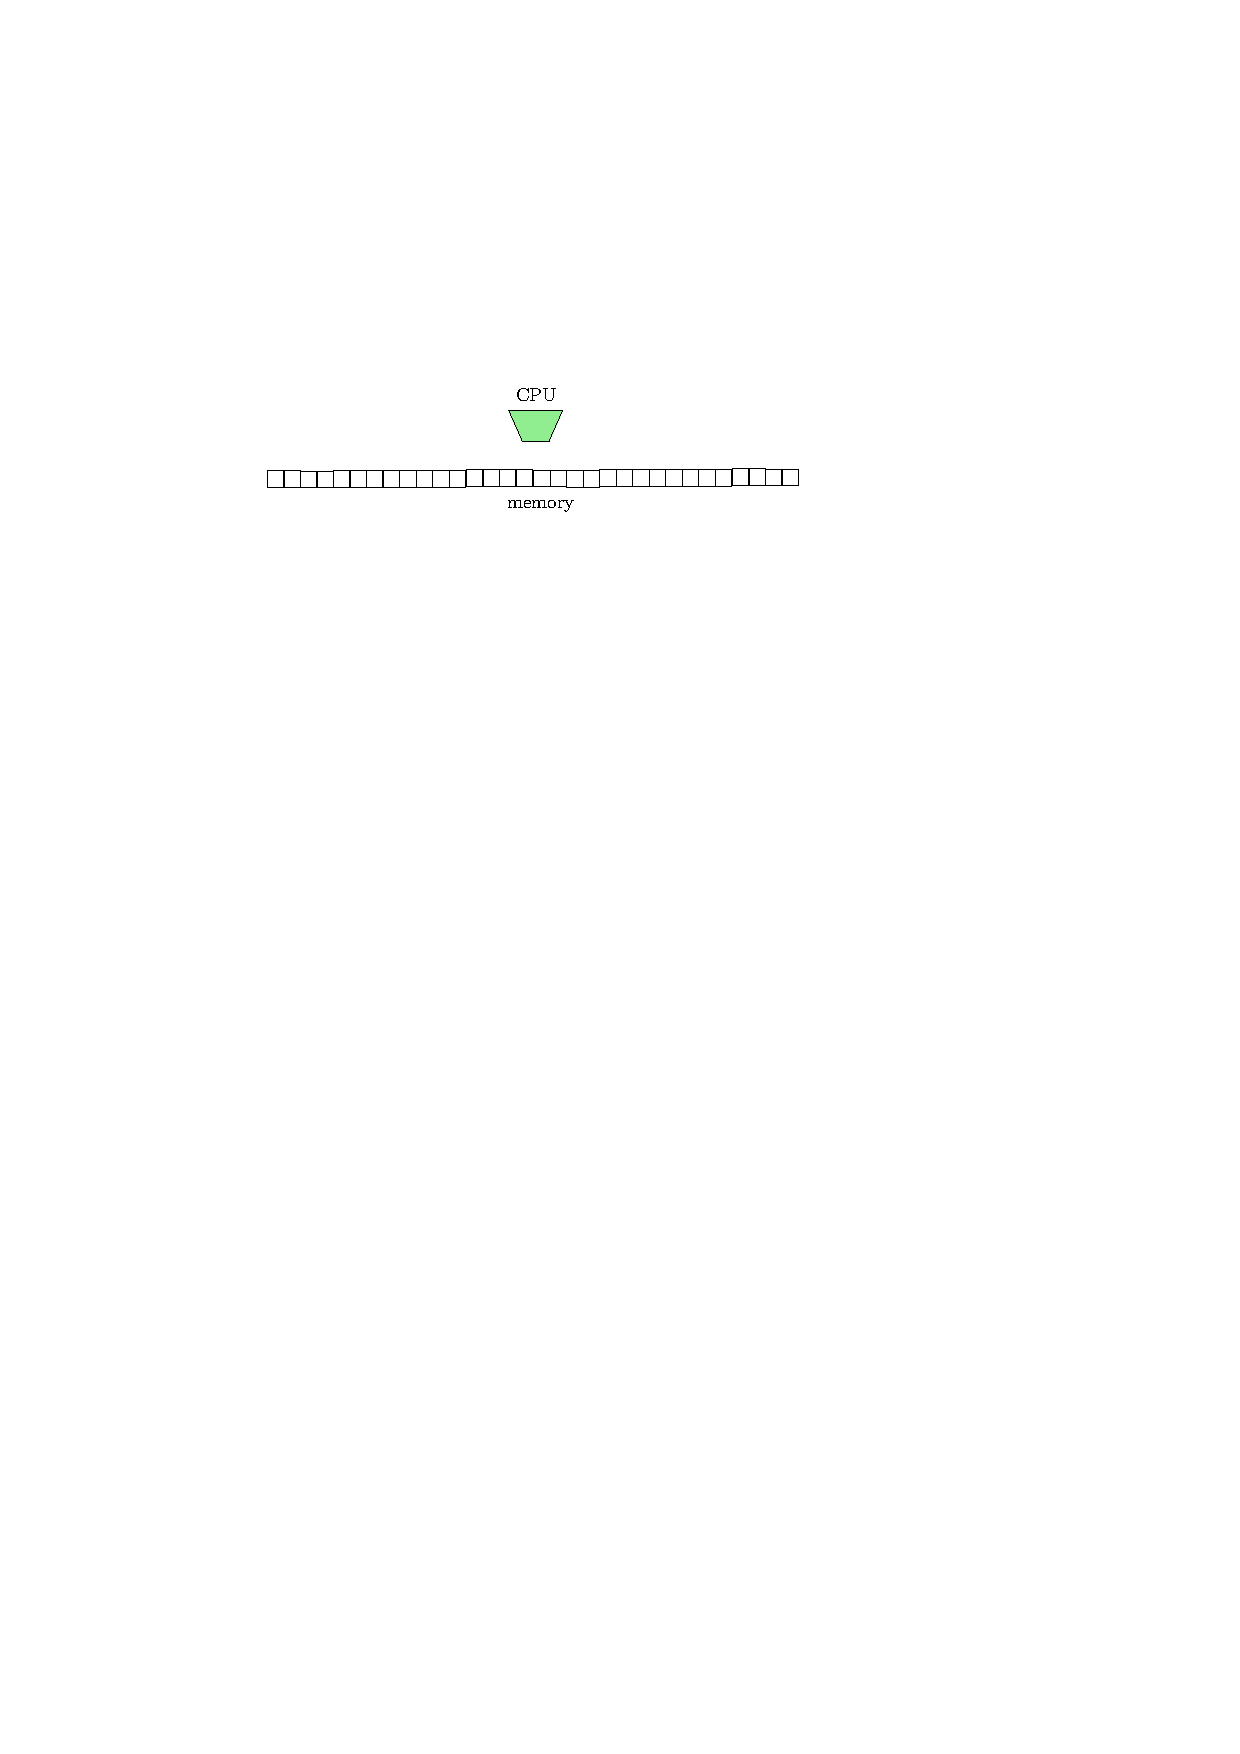
\includegraphics[height=20mm]{./artwork/ram}
	\end{center}

	\blue{Atomic operations} ($\red{a}$ and $\red{b}$ are registers):
	\myitems{
		\item $a \leftarrow 100$, $a \leftarrow b$
		\item $a + b$, $a - b$, $a * b$, $a / b$
		\item $a < b$, $a = b$, or $a > b$
		\item read a memory cell into $a$, or write $a$ into a memory cell.
	}

	\vgap

	\blue{Time} of an algorithm = \# atomic operations performed.
}
%-------------------------------------------------------------
\myfrm{

    \cbox{blue}{
        \blue{The Sorting Problem:} Given an array \red{$A$} of \red{$n$} distinct integers, produce another array where the same integers have been arranged in ascending order.
    }
}
%-------------------------------------------------------------
\myfrm{
	\xmybox[red]{Merge Sort}

	\begin{itemize}
        \item \blue{\bf Divide:} Let $\red{A_1}$ the array containing the first $\lc n/2 \rc$ elements of $A$, and $\red{A_2}$ be the array containing the other elements of $A$. \\ Sort $A_1$ and $A_2$ recursively.

        \item \blue{\bf Conquer:} Merge the two sorted arrays $A_1$ and $A_2$ in ascending order. This can be done in $O(n)$ time.
    \end{itemize}

    \vgap

    $\red{f(n)}$: time of sorting $n$ integers
    \myeqn{
		f(n) = 2 \cdot f(n/2) + O(n) \nn
    }
    which yields $f(n) = O(n \log n)$.
}
%-------------------------------------------------------------
\myfrm{
	\cbox{red}{
		A computation model falls short when it can no longer be used to guide the design of algorithms.
	}

	\vgap

	Today, a modern CPU has multiple cores and supports \bred{parallel execution}. \\

	\vgap

	RAM can no longer capture an algorithm's behavior on those CPUs.
}
%-------------------------------------------------------------
\myfrm{
	\cbox{yellow}{
	\centering
		II. Parallel Random Access Machine (PRAM)
	}
}
%-------------------------------------------------------------
\myfrm{
	$\red{p}$ = \# CPUs

	\begin{center}
	    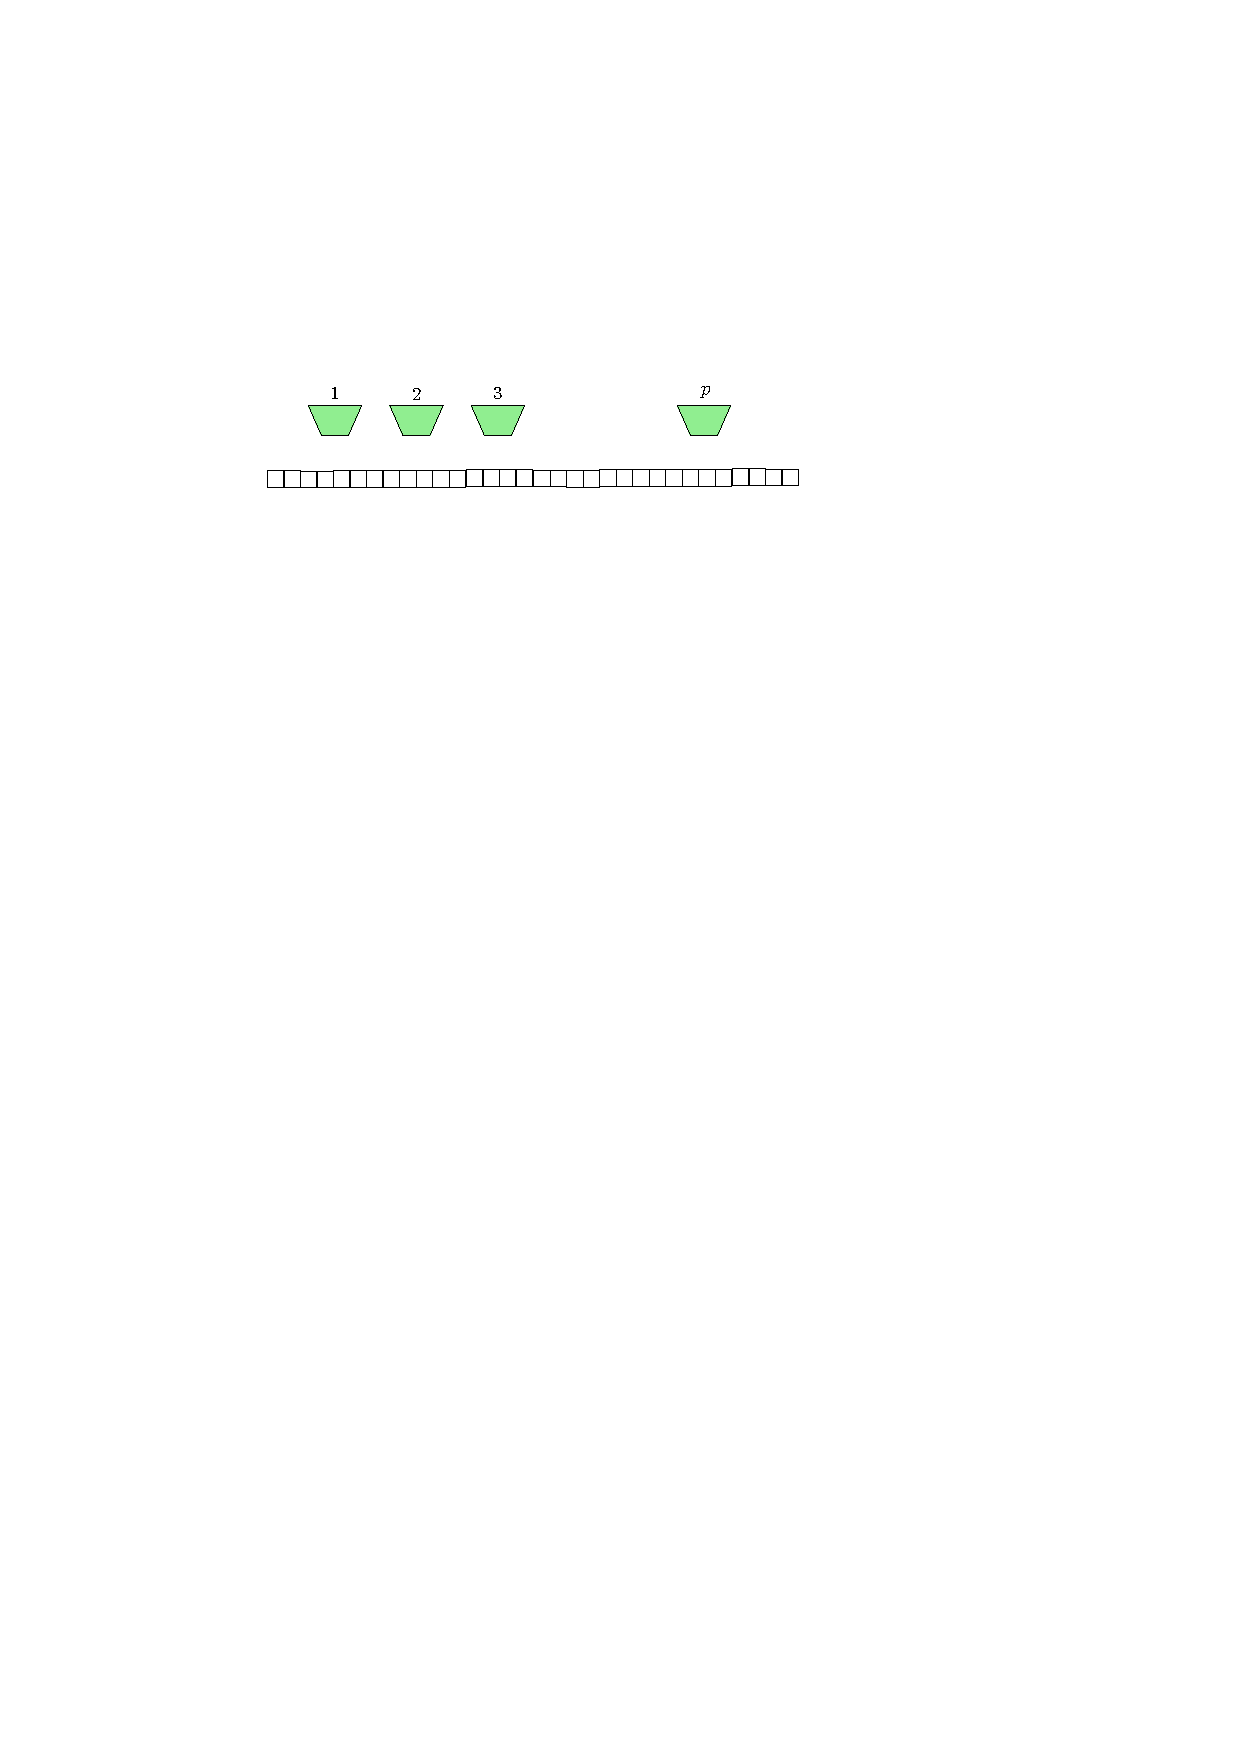
\includegraphics[height=13mm]{./artwork/pram}
	\end{center}

	A \blue{step}: each CPU \red{independently} performs an atomic operation ($\red{a}$ and $\red{b}$ are registers inside the CPU):
	\myitems{
		\item $a \leftarrow 100$, $a \leftarrow b$
		\item $a + b$, $a - b$, $a * b$, $a / b$
		\item $a < b$, $a = b$, or $a > b$
		\item read a memory cell into $a$, or write $a$ into a memory cell.
	}

	\cbox{blue}{
		\blue{Constraint:} In a step, if a CPU writes to a cell, no other CPU can read or write to the cell.
	}

	This is the \blue{CREW} model (common read exclusive write).
}
%-------------------------------------------------------------
\myfrm{

    \cbox{blue}{
        \blue{The Sorting Problem:} Given an array \red{$A$} of $\red{n} \ge p$ distinct integers, produce another array where the same integers have been arranged in ascending order.
    }

    %\vgap

    \begin{center}
	    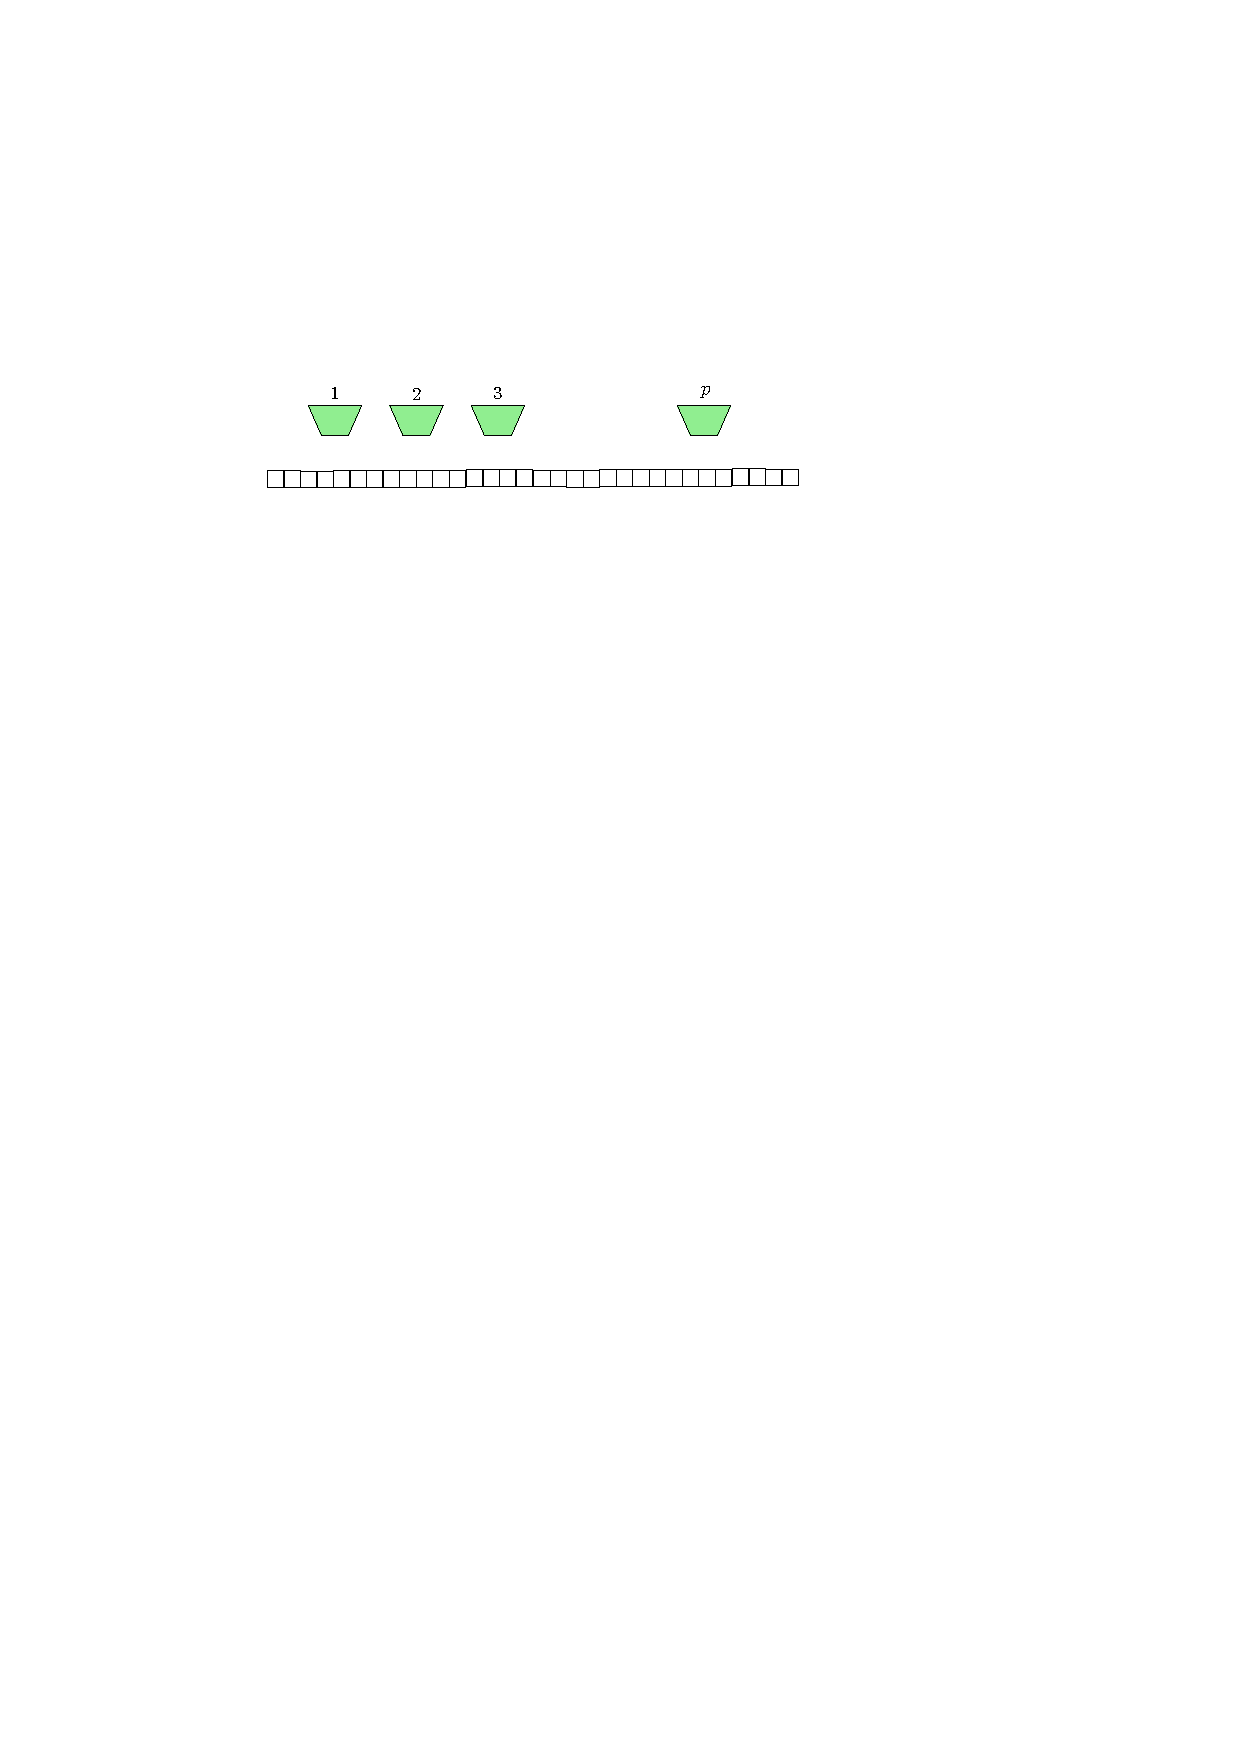
\includegraphics[height=13mm]{./artwork/pram}
	\end{center}

	Naive: $O(n \log n)$ steps. \\
	Optimal: $O(\fr{n}{p} \log n)$ steps. \bred{Why?} \\

	\vgap

	We will see how to do $O(\red{\fr{n}{p} \log^2 n})$ steps. \\

	\vgap

	We will assume $p = n$. Extending the discussion to $p < n$ is left to you.
}
%-------------------------------------------------------------
\myfrm{
	\cbox{blue}{
        \blue{The Merging Problem:} Let $\red{A_1}$ and $\red{A_2}$ be two sorted arrays, each with $p/2$ integers. Merge $A_1$ and $A_2$ into one sorted array (with $p$ integers).
    }

    \vgap

    Naive: $O(p)$ steps. \\
    We will do $O(\log p)$ steps.
}
%-------------------------------------------------------------
\myfrm{
	%\xmybox[red]{Idea}

	\begin{center}
	    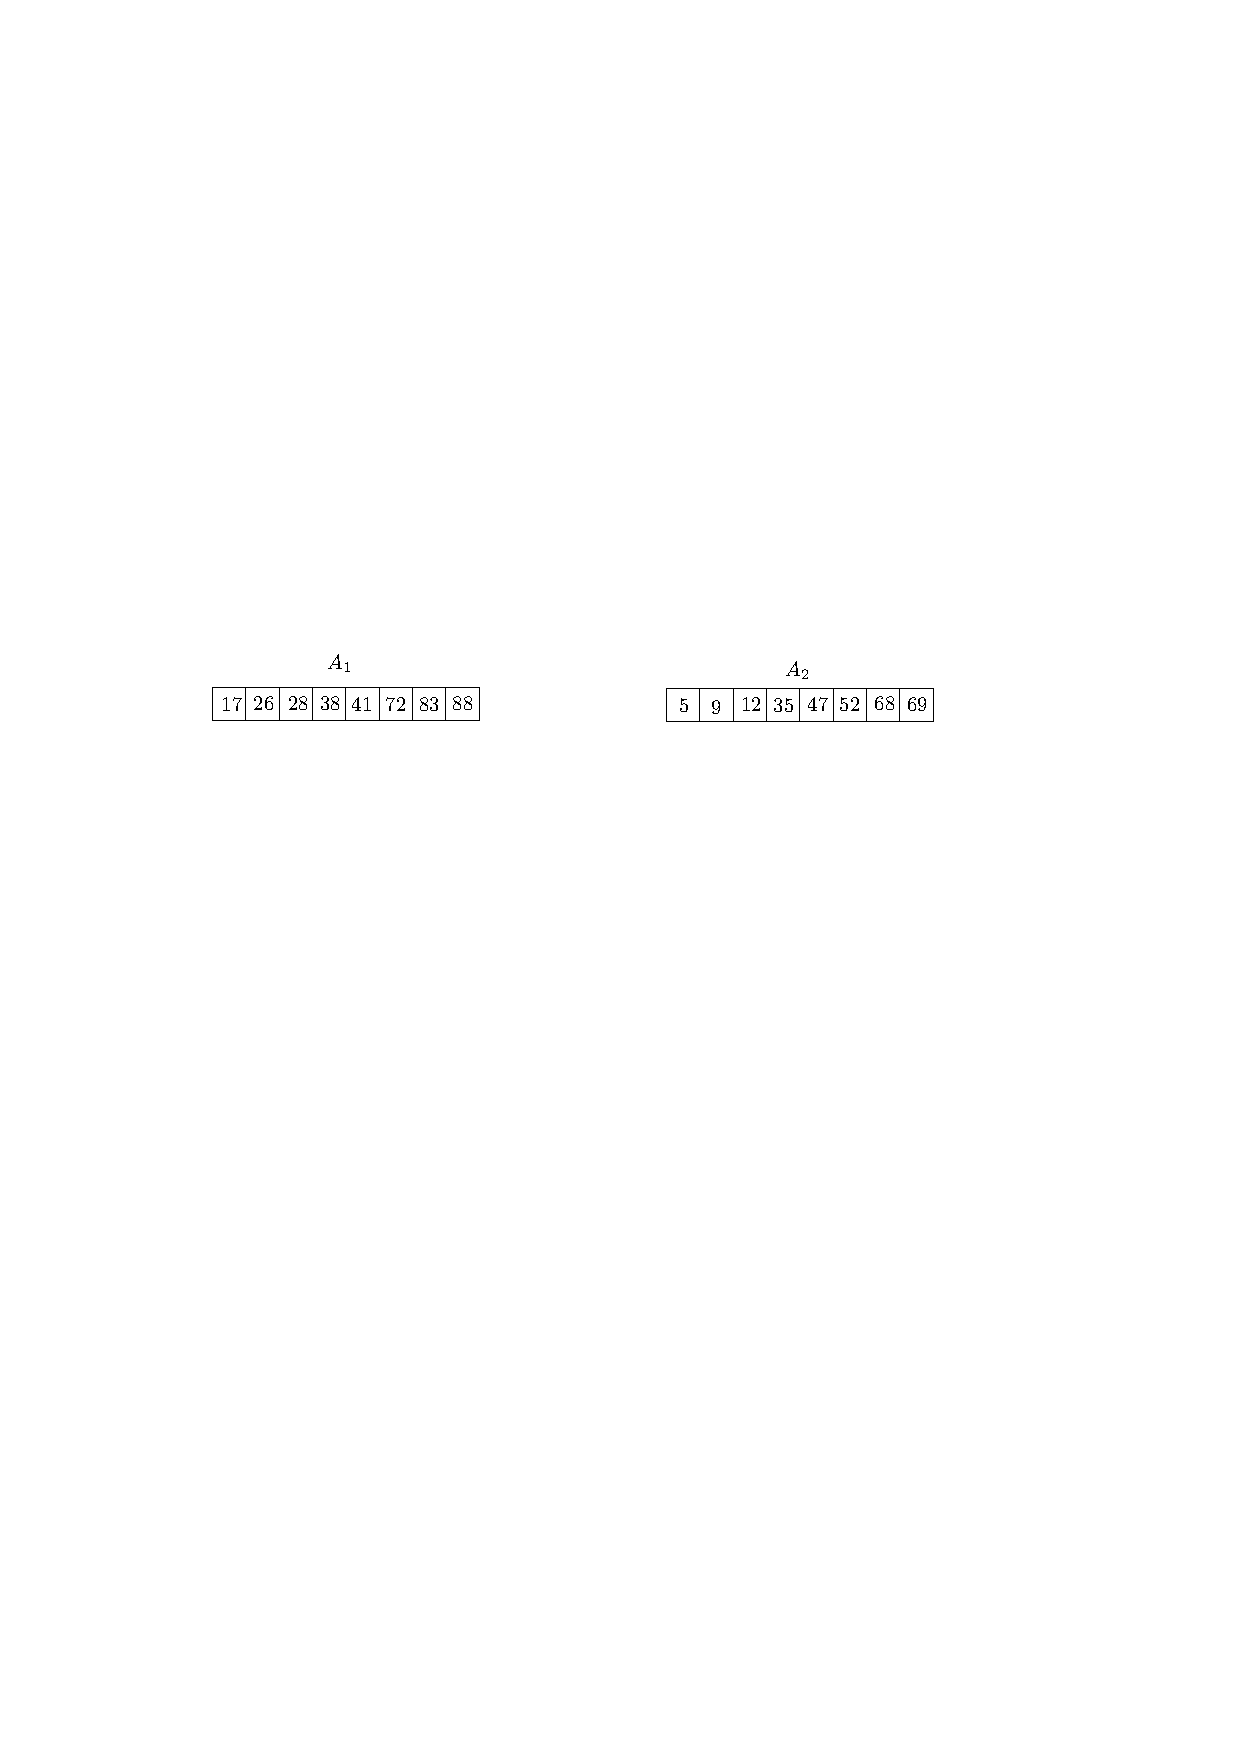
\includegraphics[height=9mm]{./artwork/merge}
	\end{center}

	Consider the number \red{26} in $A_1$.
	\myitems{
		\item It is the 2nd smallest in $A_1$.
		\item It is greater than 3 numbers in $A_2$.
	}
	Hence, 26 should be the $2 + 3 = 5$-th in the merged array.
}
%-------------------------------------------------------------
\myfrm{
	%\xmybox[red]{Idea}

	\begin{center}
	    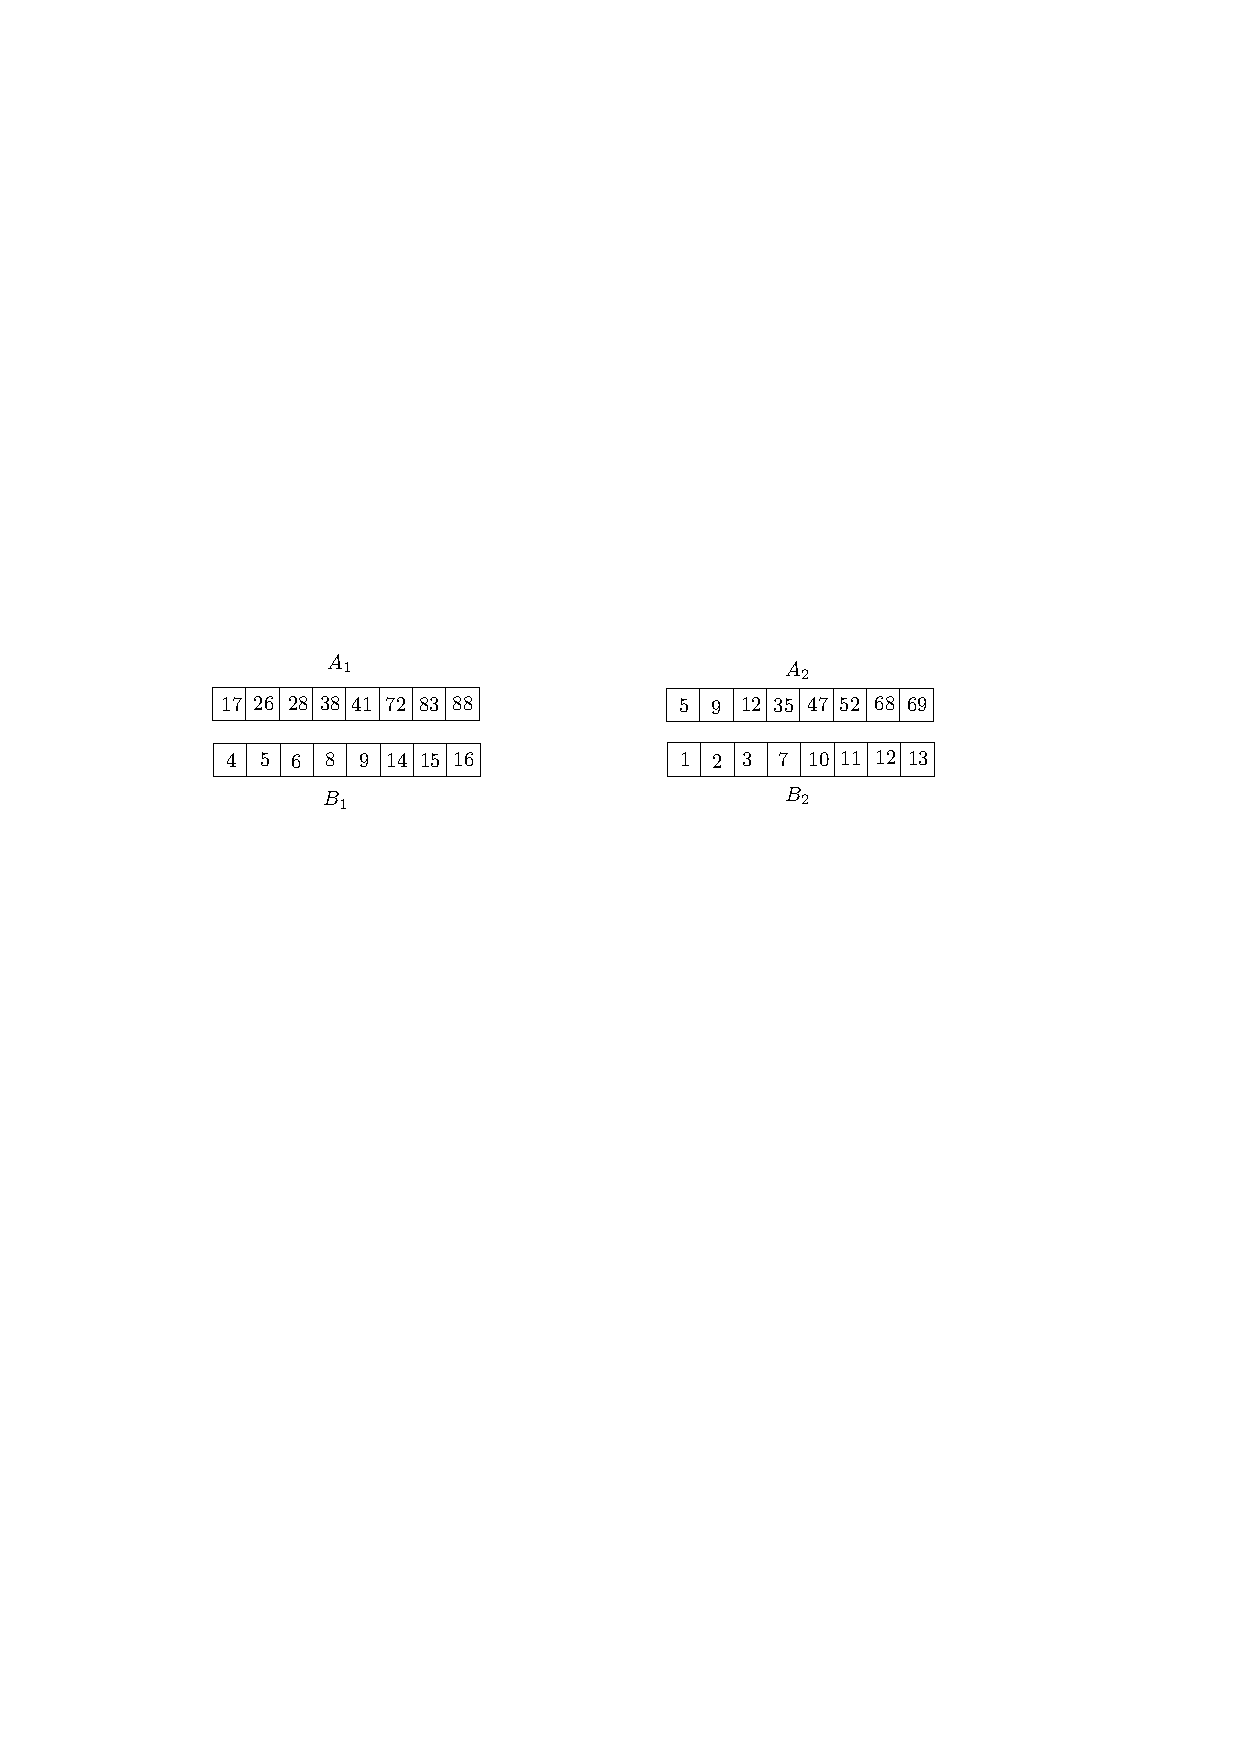
\includegraphics[height=20mm]{./artwork/merge2}
	\end{center}

	We want to generate arrays $\red{B_1}$ and $\red{B_2}$. For each number $\red{x}$ in $A_1$ (or $A_2$), the corresponding cell in $B_1$ (or $B_2$) indicates the position of $x$ in the final merged array.

	\vgap

	Once $B_1$ and $B_2$ are ready, the merged array can be produced in $O(1)$ steps --- recall that we have $p = 16$ CPUs.
}
%-------------------------------------------------------------
\myfrm{
	%\xmybox[red]{Idea}

	\begin{center}
	    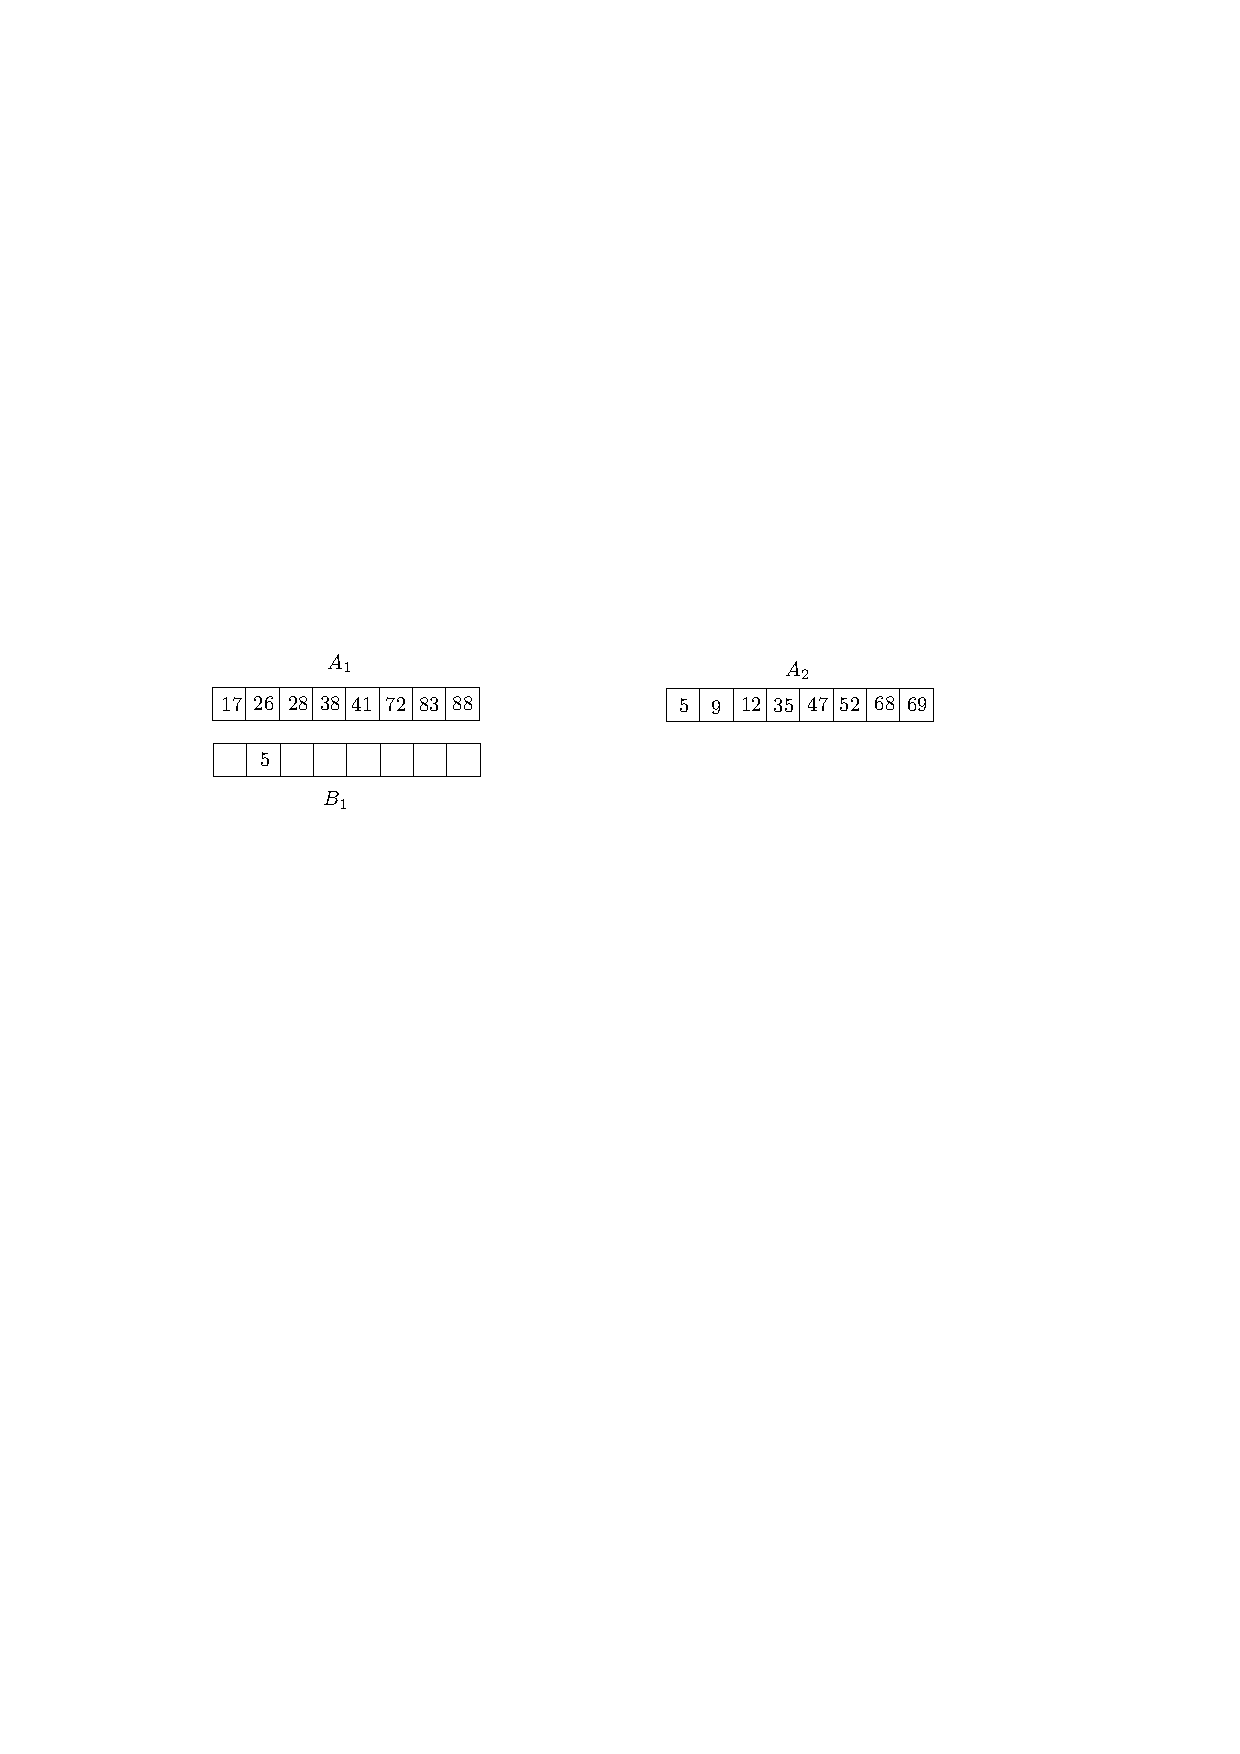
\includegraphics[height=20mm]{./artwork/merge3}
	\end{center}

	How to generate $B_1$ and $B_2$? \\

	By assigning one CPU to each number, we can generate the number's position indicator in $O(\log p)$ steps using binary search.

	\vgap

	This gives an algorithm solving the merging problem in $O(\log p)$ steps.
}
%-------------------------------------------------------------
\myfrm{
	We can now sort $n$ elements with $n$ CPUs in $O(\log n)$ phases.

	\myitems{
		\item Phase 0: $n/2$ parallel merges, each merging two lists of size 1.
		\item Phase 1: $n/4$ parallel merges, each merging two lists of size 2.
		\item Phase 2: $n/8$ parallel merges, each merging two lists of size 4.
		\item ...
	}

	Each phase takes $O(\log n)$ steps. \\
	Overall, $O(\log^2 n)$ steps.
}
%-------------------------------------------------------------
\myfrm{
	\cbox{yellow}{
	\centering
		III. External Memory (EM)
	}
}
%-------------------------------------------------------------
\myfrm{
	RAM and PRAM assume that the data fit in memory.

	\vgap

	In practice, a dataset often needs to be stored in the disk. In those scenarios, CPU operations are rarely the performance bottleneck. Typically, an algorithm's efficiency depends on how many \bred{disk I/Os} are performed.

	\vgap

	This motivates the \blue{external memory} model.
}
%-------------------------------------------------------------
\myfrm{
	$\red{M}$ = the number of words in memory \\
	$\red{B}$ = the number of words in a disk block

	\begin{center}
	    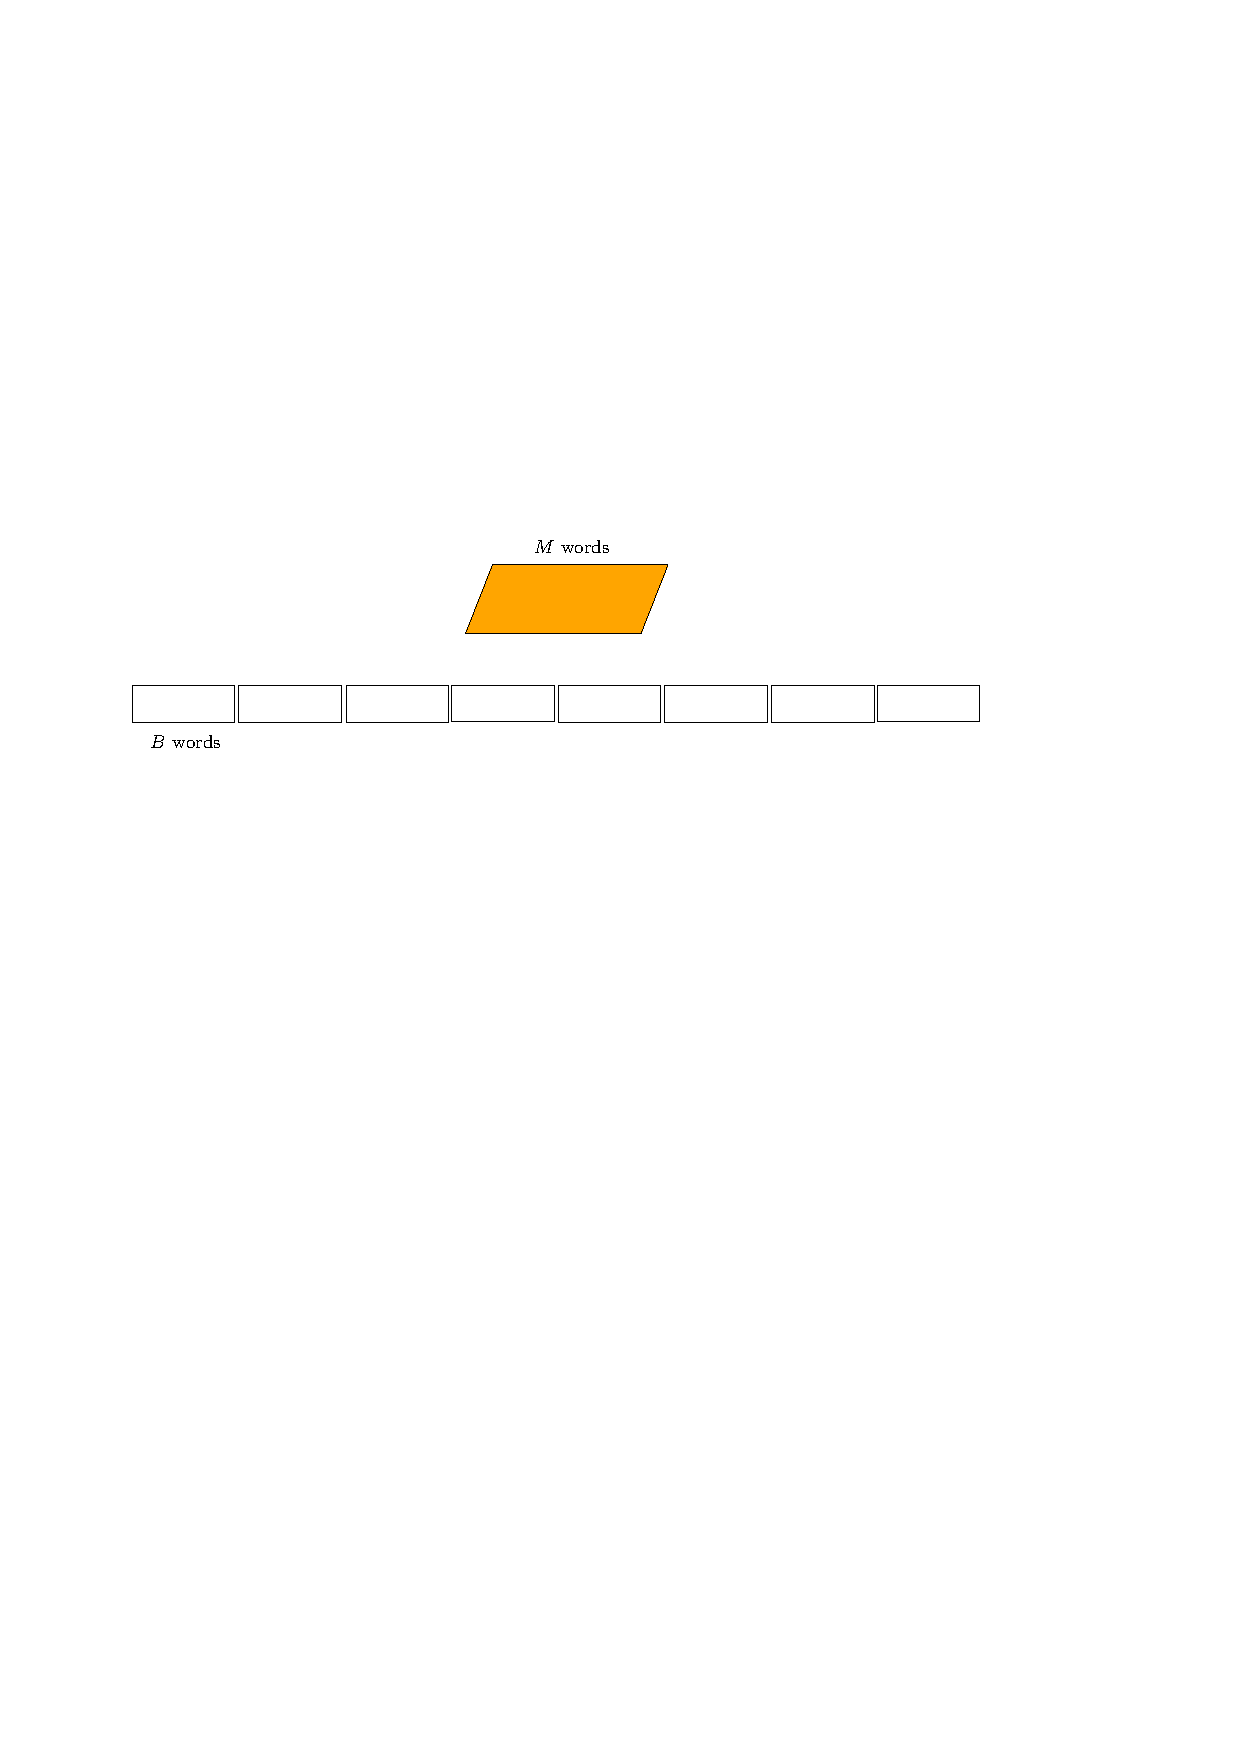
\includegraphics[height=24mm]{./artwork/em}
	\end{center}

	\vgap

	A \blue{I/O}
	\myitems{
		\item reads a disk block into memory, or
		\item writes $B$ memory words into a disk block.
	}
	\blue{Cost} of an algorithm: \# I/Os performed.

	\vgap

	\cbox{blue}{
		CPU calculation is for free.
	}
}
%-------------------------------------------------------------
\myfrm{

	\cbox{blue}{
        \blue{The Sorting Problem:} Given a file \red{$A$} of $\red{n} \ge B$ distinct integers stored in $O(n/B)$ blocks, produce another file of $O(n/B)$ blocks where the same integers have been arranged in ascending order.
    }

    \vgap

    Naive: $O(n \log n)$ I/Os. \\
    We will do: $O(\fr{n}{B} \log_{M/B} \fr{n}{B})$ I/Os. \\
}
%-------------------------------------------------------------
\myfrm{

	\cbox{blue}{
        \blue{The Merging Problem:}
        Let \red{$A_1$}, $\red{A_2}$, ..., $\red{A_{\fr{M}{B}-1}}$ be $\fr{M}{B}-1$ files such that
        \myitems{
			\item each file stores $\red{t_i} \ge B$ integers in ascending order with $O(\red{t_i} / B)$ block;
			\item the integers in all the files are distinct.
        }
		Let $\red{t} = \sum_{i=1}^{M/B-1} t_i$. Produce another file of $O(t/B)$ blocks where all the $t$ integers have been arranged in ascending order.
    }

    \vgap

    We will see how to solve the problem in $O(t/B)$ I/Os.
}
%-------------------------------------------------------------
\myfrm{
	\begin{center}
	    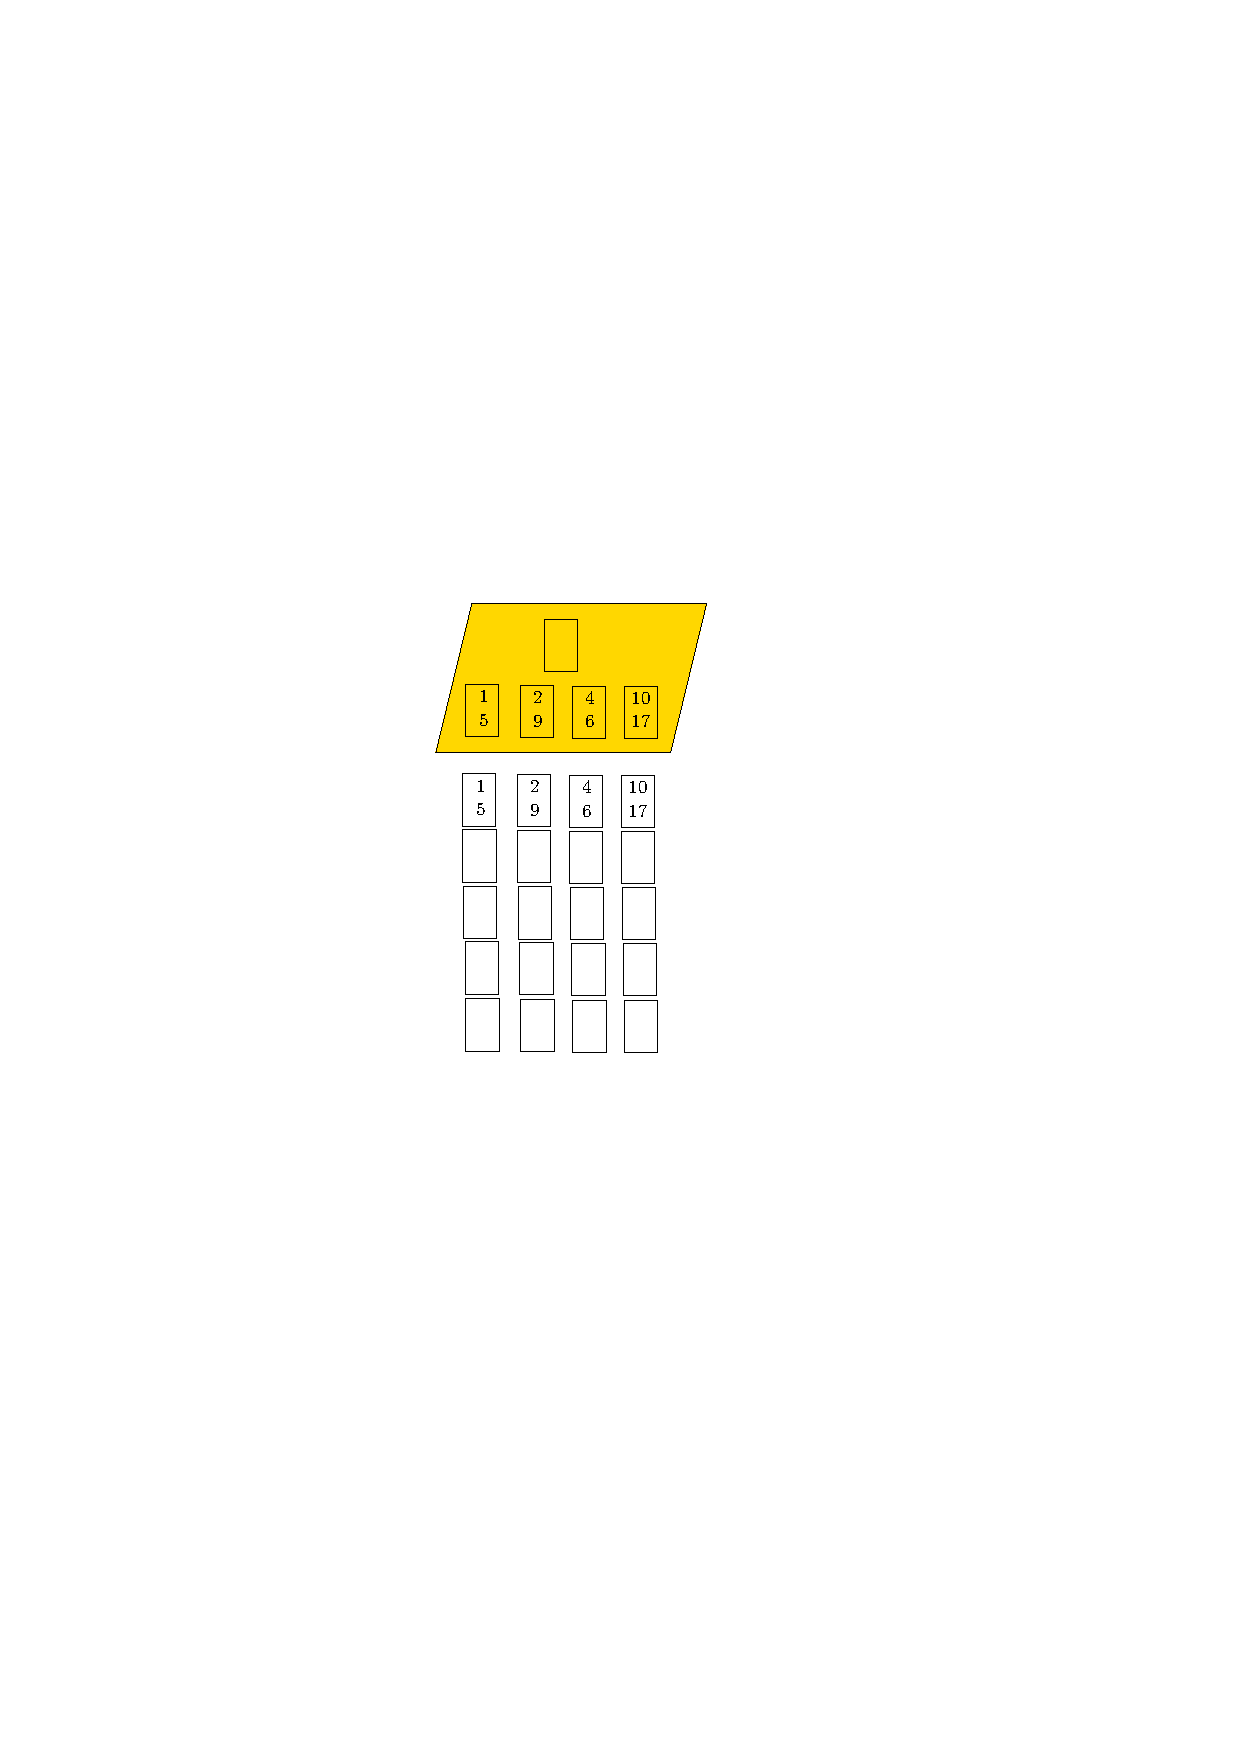
\includegraphics[height=60mm]{./artwork/em-merge}
	\end{center}
}
%-------------------------------------------------------------
\myfrm{
	\begin{center}
	    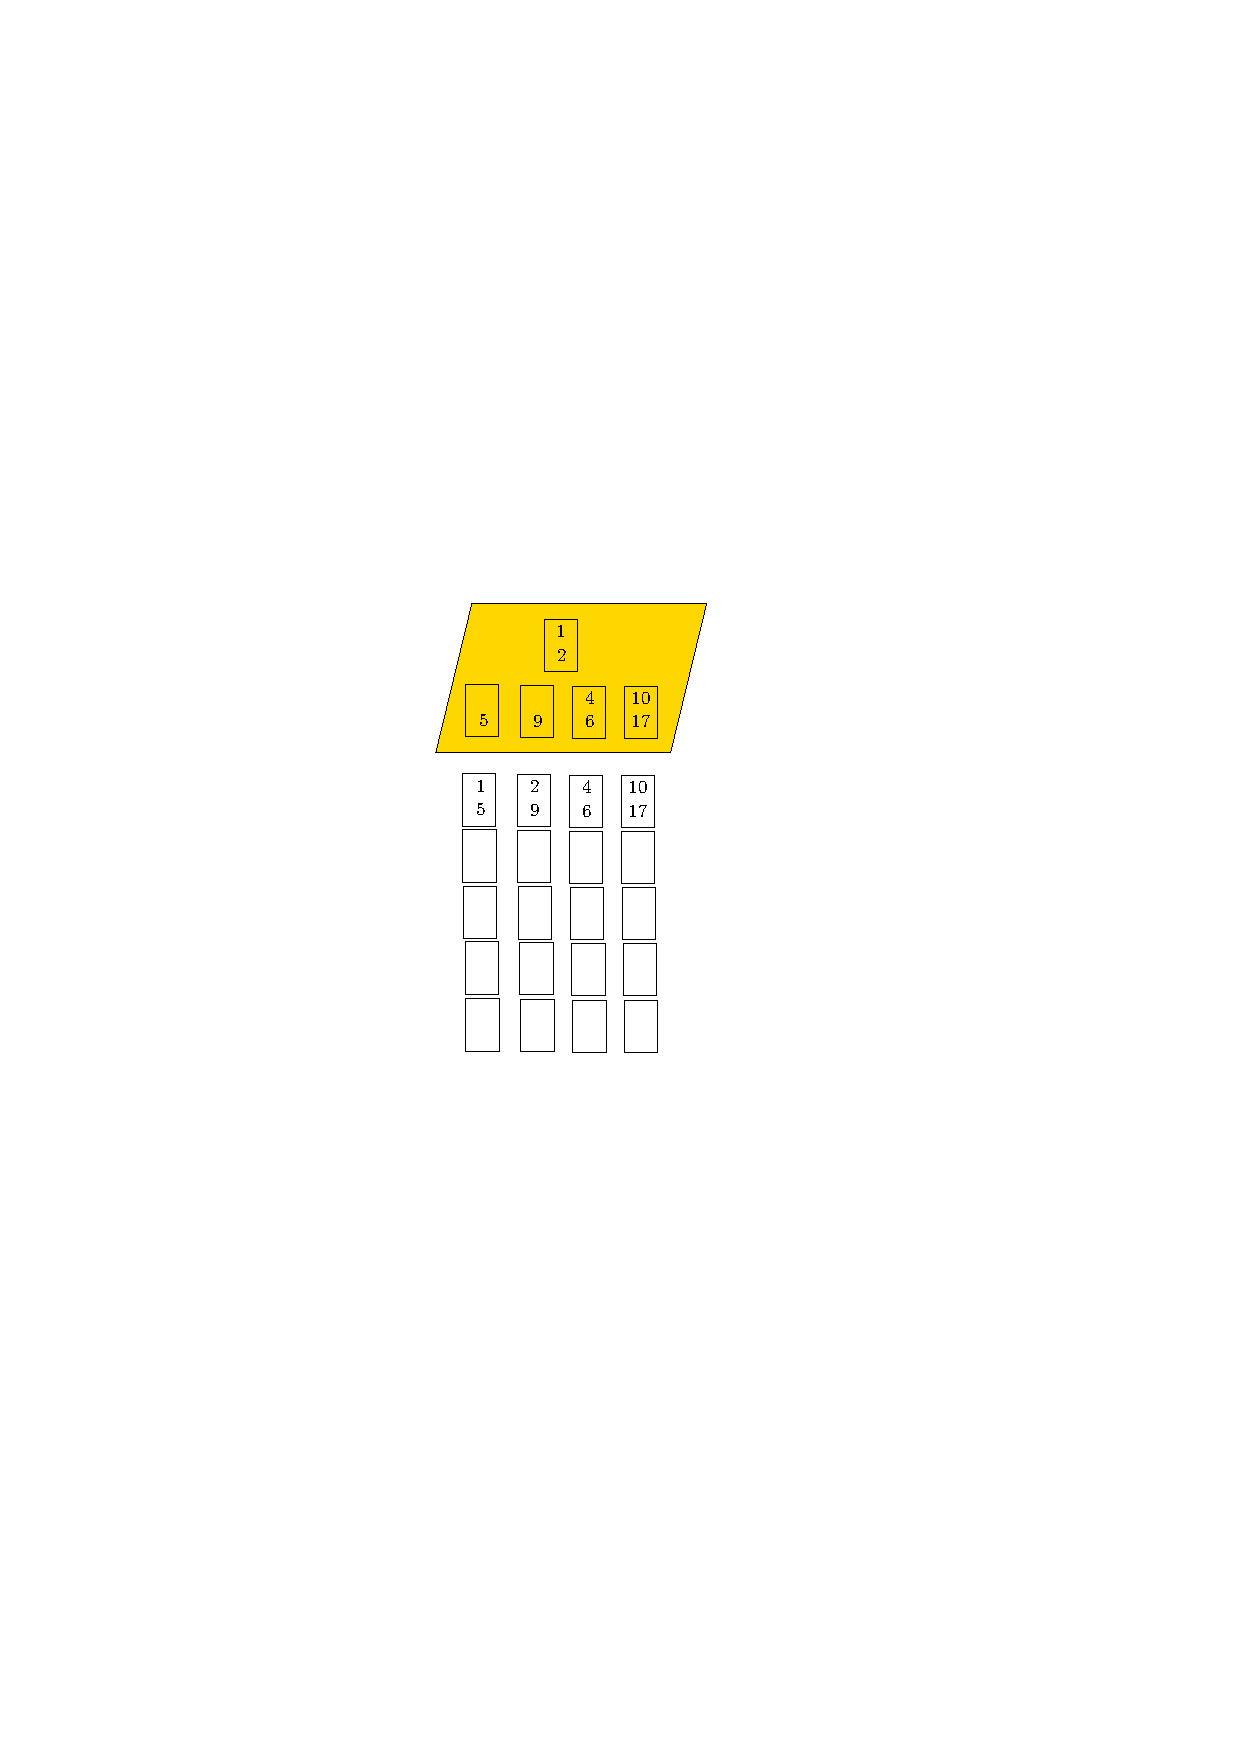
\includegraphics[height=60mm]{./artwork/em-merge2}
	\end{center}
}
%-------------------------------------------------------------
\myfrm{
	\begin{center}
	    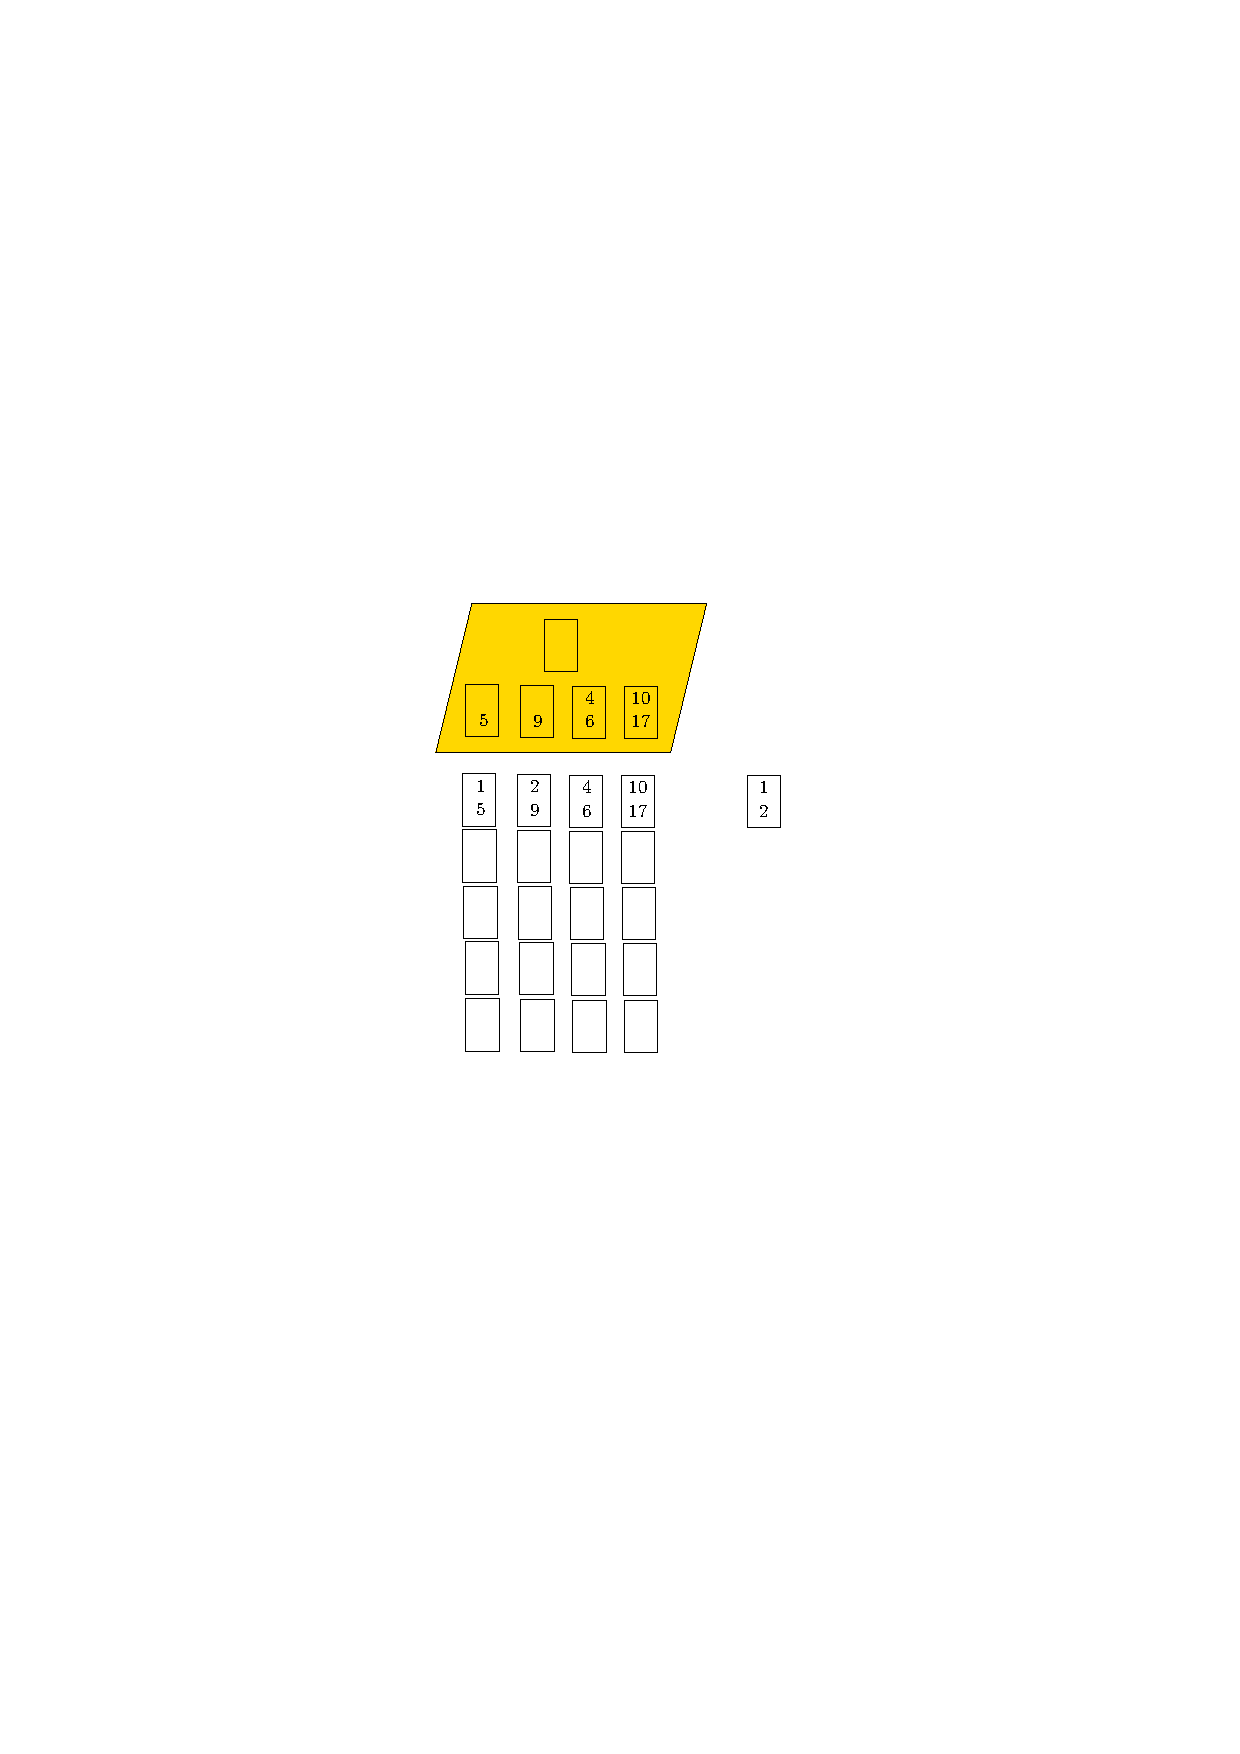
\includegraphics[height=60mm]{./artwork/em-merge3}
	\end{center}
}
%-------------------------------------------------------------
\myfrm{
	\begin{center}
	    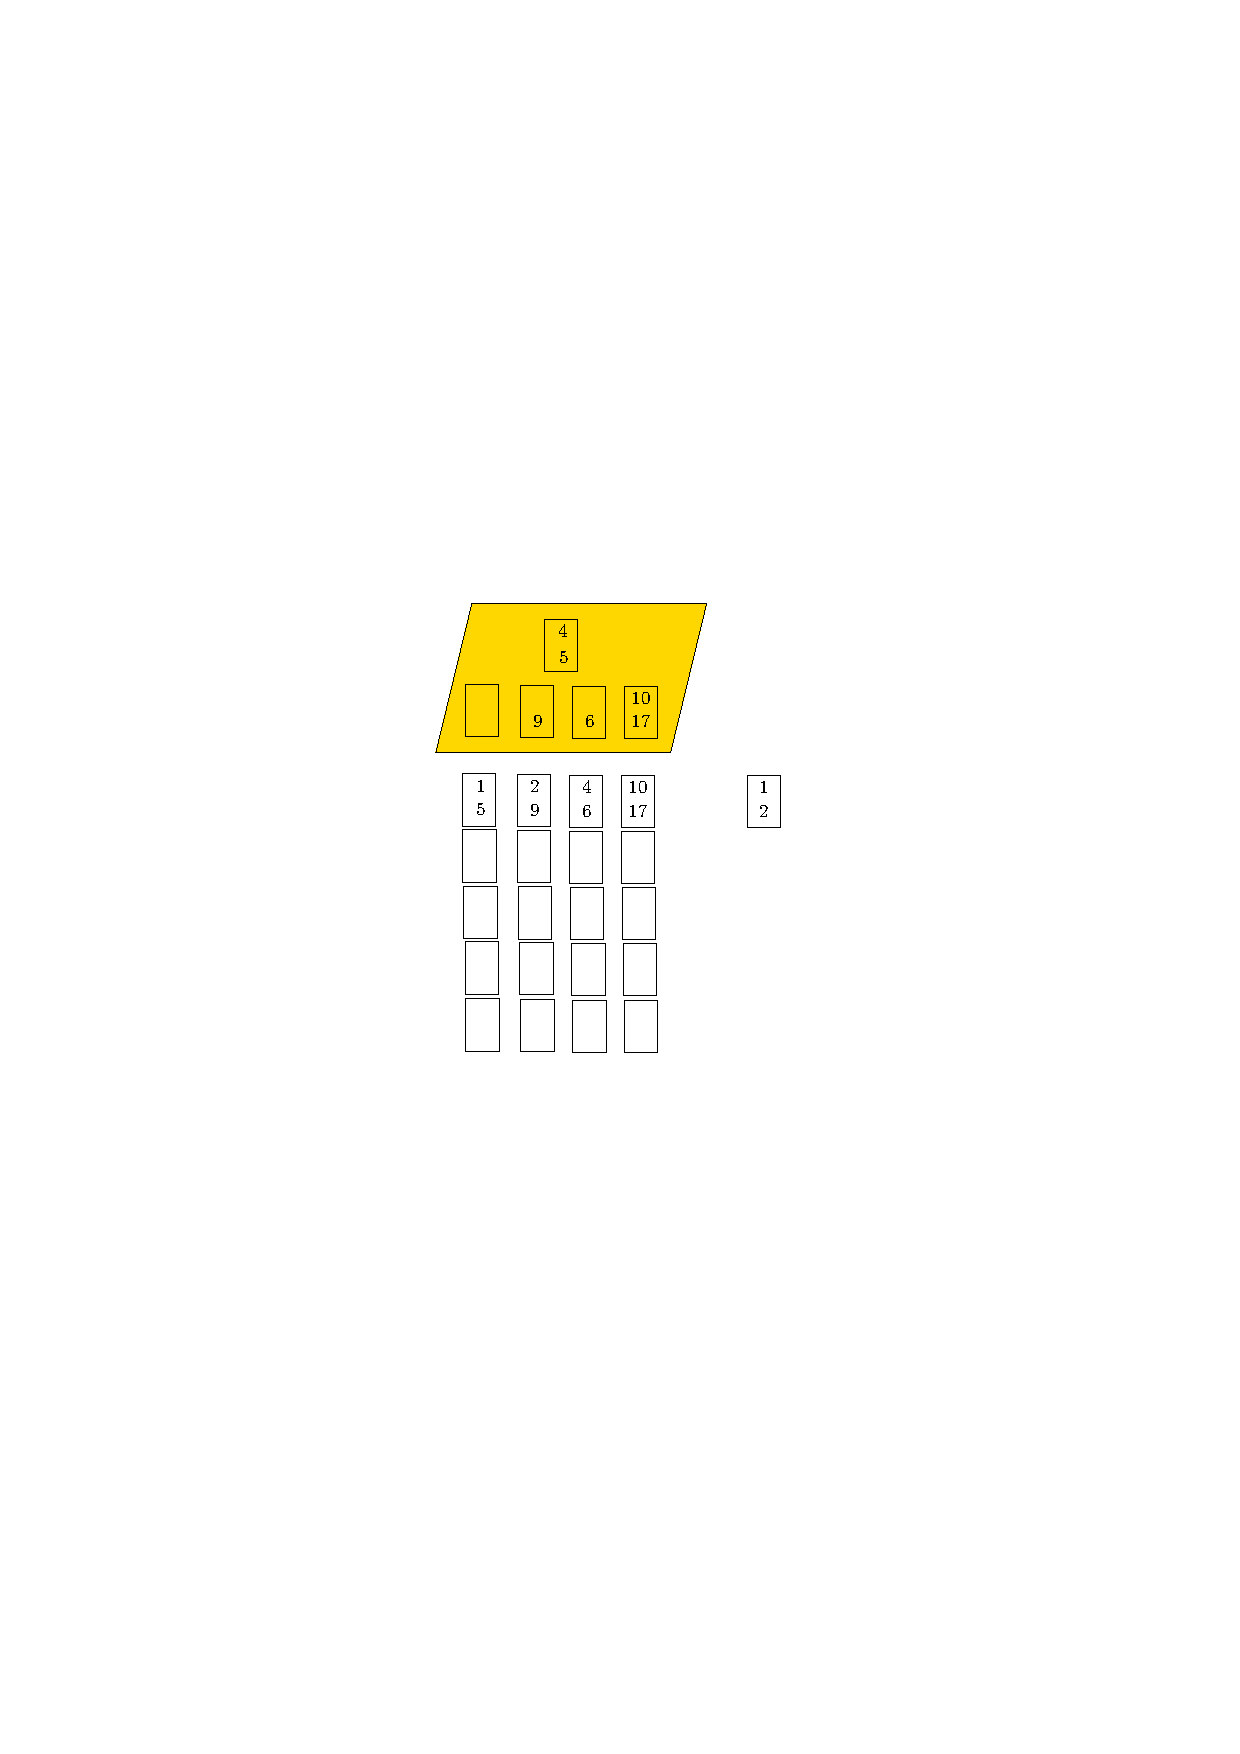
\includegraphics[height=60mm]{./artwork/em-merge4}
	\end{center}
}
%-------------------------------------------------------------
\myfrm{
	\begin{center}
	    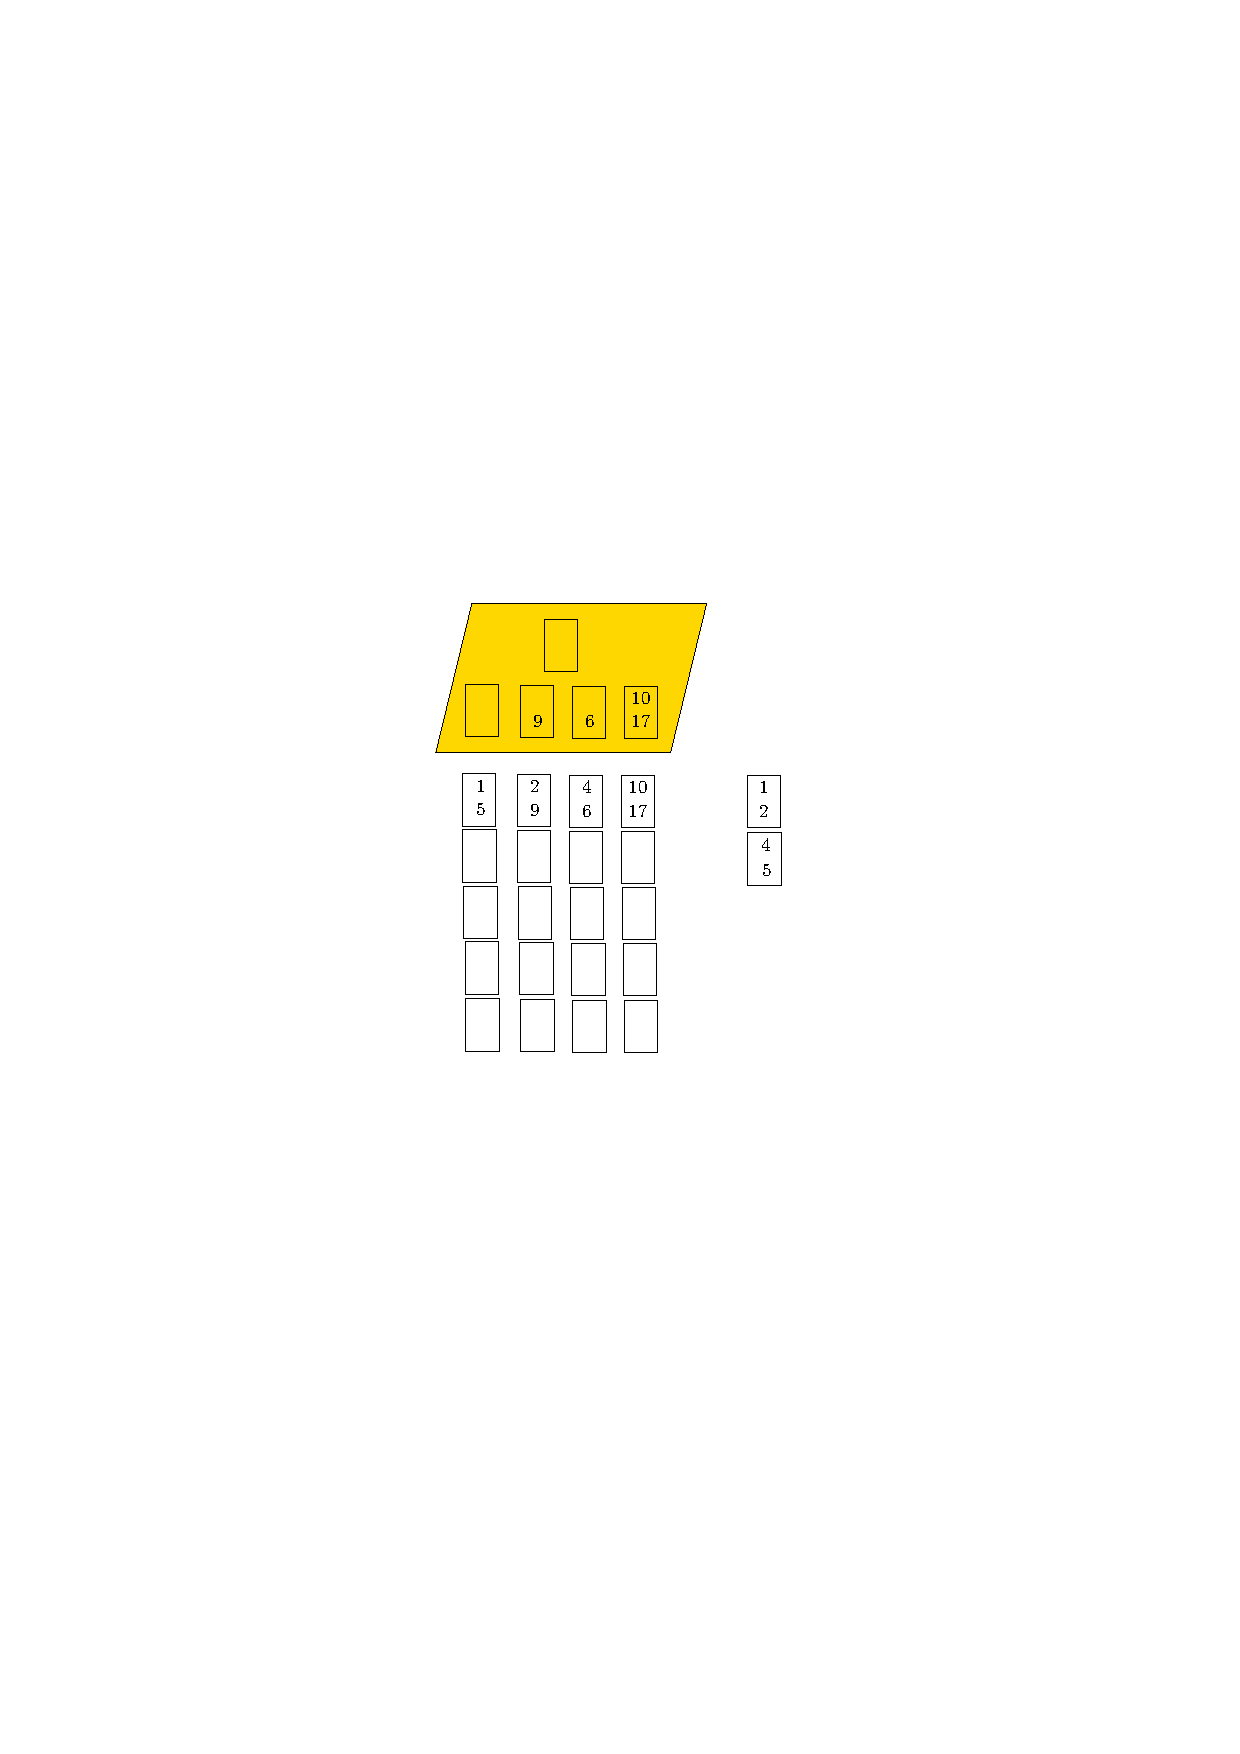
\includegraphics[height=60mm]{./artwork/em-merge5}
	\end{center}
}
%-------------------------------------------------------------
\myfrm{
	\begin{center}
	    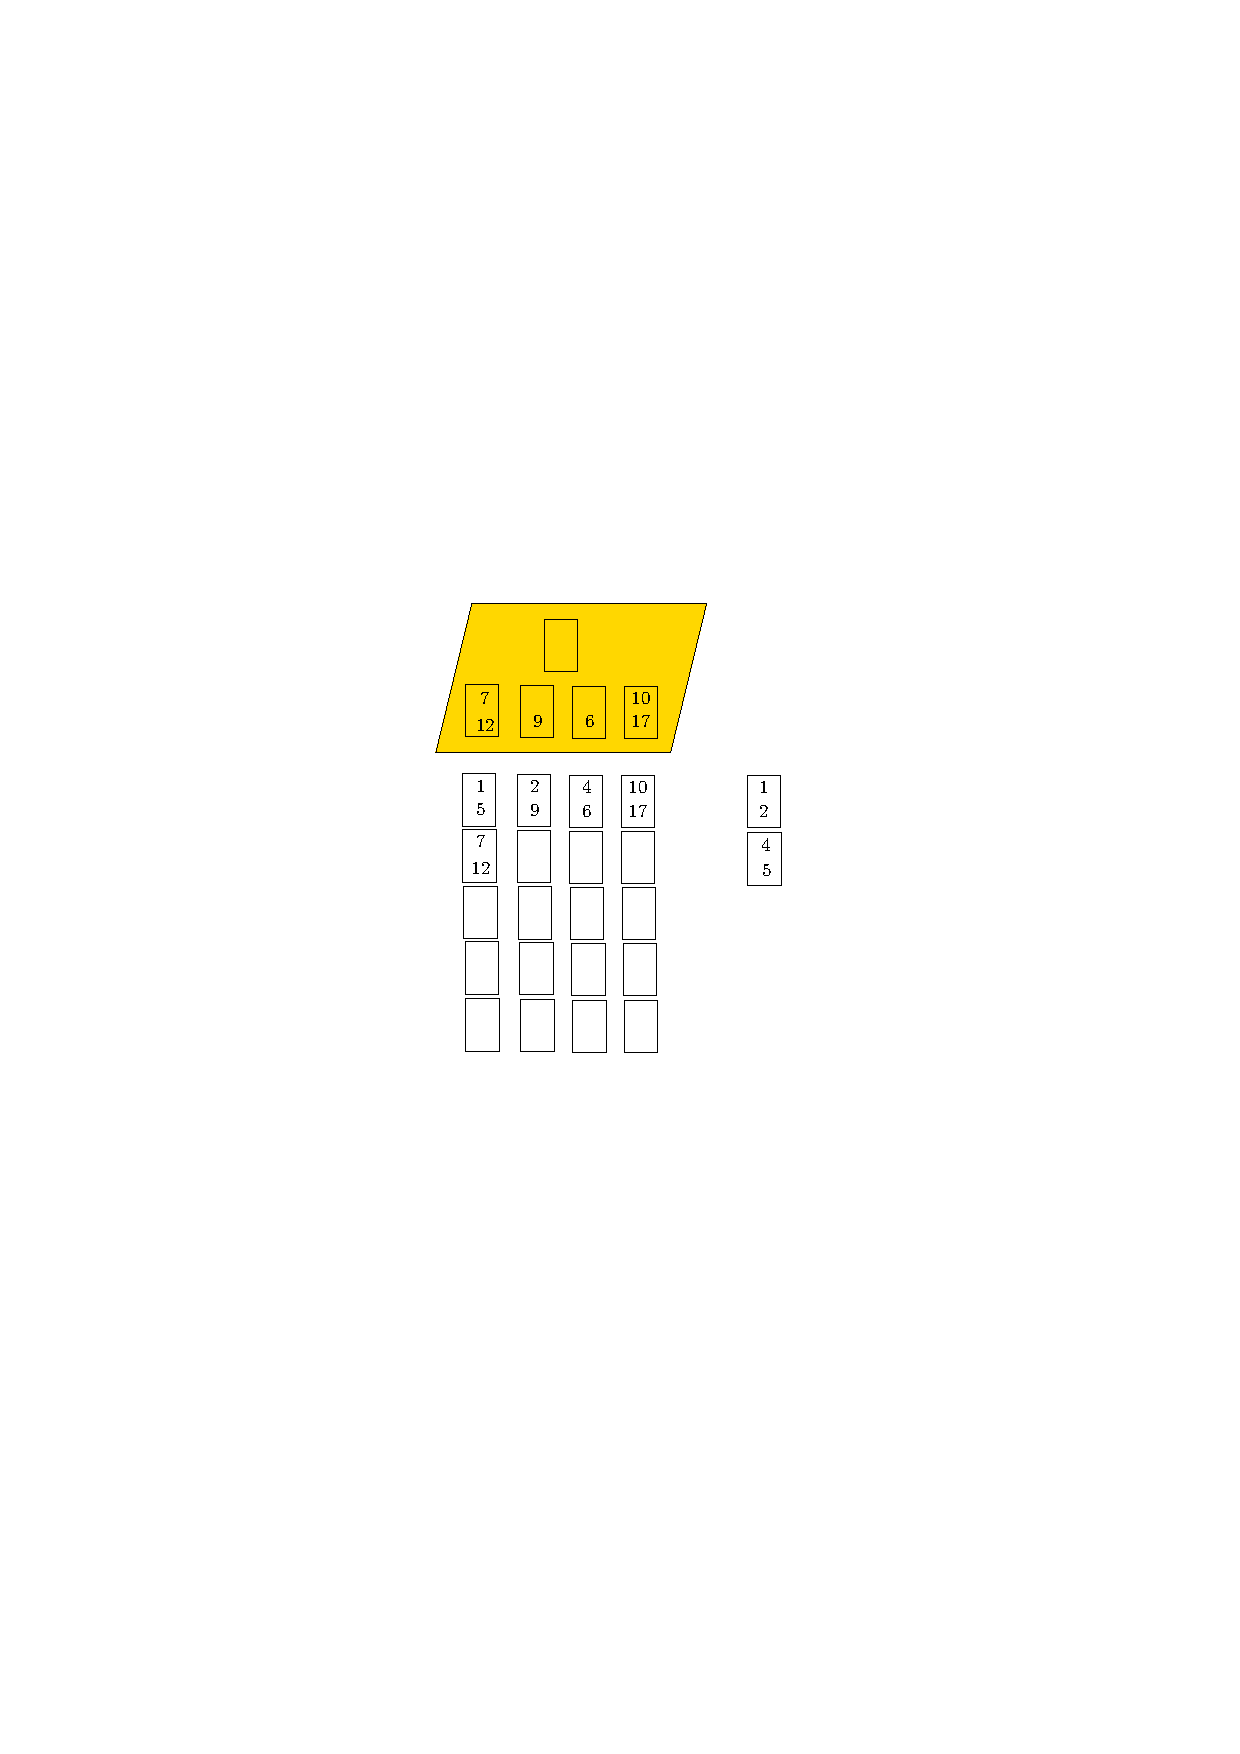
\includegraphics[height=60mm]{./artwork/em-merge6}
	\end{center}

	The total cost is $O(t/B)$ because
	\myitems{
		\item there are $O(t/B)$ blocks in the input files;
		\item there are $O(t/B)$ blocks in the output file.
	}
}
%-------------------------------------------------------------
\myfrm{
	Think: equipped with the above merging algorithm, how can we solve the sorting problem in $O(\fr{n}{B} \log_{M/B} \fr{n}{B})$ I/Os?
}
%-------------------------------------------------------------
\myfrm{
	\cbox{yellow}{
	\centering
		IV. Massively Parallel Computation (MPC)
	}
}
%-------------------------------------------------------------
\myfrm{
	Today, many computational tasks are performed on datasets whose sizes are at the tera-byte order or higher. Massively-parallel systems (such as Spark) are often deployed to carry out those tasks. Such a system involves dozens or hundreds of machines interconnected by a broadband network. CPU time and I/O cost are no longer the performance bottleneck. Instead, the efficiency of an algorithm is determined by \bred{network communication}.

	\vgap

	This motivates the \blue{massively parallel computation} (MPC) model.
}
%-------------------------------------------------------------
\myfrm{
	$\red{p}$ = \# machines

	\vgap

	A \blue{superstep} includes two steps.
	\myitems{
		\item Step 1: each machines performs local computation.

		\item Step 2: each machine sends a message to every other machine.
	}

	\vgap

	\blue{Cost of a superstep:} the maximum number of words communicated (i.e., sent and received) by a machine in Step 2.
	\myitems{
		\item Step 1 is for free.
	}

	\vgap

	\blue{Cost of an algorithm:} total cost of all the supersteps.
}
%-------------------------------------------------------------
\myfrm{
	\cbox{green}{
		\blue{Example:}

		$p = 3$ machines. Suppose that in a superstep
		\myitems{
			\item machine 1 sends 50m and 30m words to machine 2 and 3, respectively;
			\item machine 2 sends 0m and 40m words to machine 1 and 3, respectively;
			\item machine 3 sends 10m and 5m words to machine 1 and 2, respectively.
		}
		Cost of the superstep = 85m words.
	}
}
%-------------------------------------------------------------
\myfrm{
	\cbox{blue}{
		\blue{The Sorting Problem:} Let $\red{S}$ be a set of $\red{n}$ numbers such that each machine stores $O(n/p)$ numbers originally. Re-arrange the numbers such that
		\myitems{
			\item each machine still stores $O(n/p)$ numbers;
			\item for any $1 \le \red{i} < \red{j} \le p$, all the numbers on machine $i$ are less than those on machine $j$.
		}
	}

	We will consider $n \ge p^3$ (a reasonable assumption in practice).

	\vgap

	Naive: cost $O(n)$. \\
	We will do: cost $O(n/p)$ in two supersteps.
}
%-------------------------------------------------------------
\begin{frame}
\begin{small}
	$\red{S_i}$ = the set of numbers on machine $i \in [1, p]$

	\vgap

    \mybox[green]{Superstep 1}


    \begin{itemize}
        \item \blue{Step 1:} Machine $\red{i}$ samples each integer in $S_i$ with probability \red{$ \fr{p}{n} \ln (np)$} independently.

        \item \blue{Step 2:} Each machine sends the samples to all other machines.

    \end{itemize}

    \vgap

    \begin{center}
        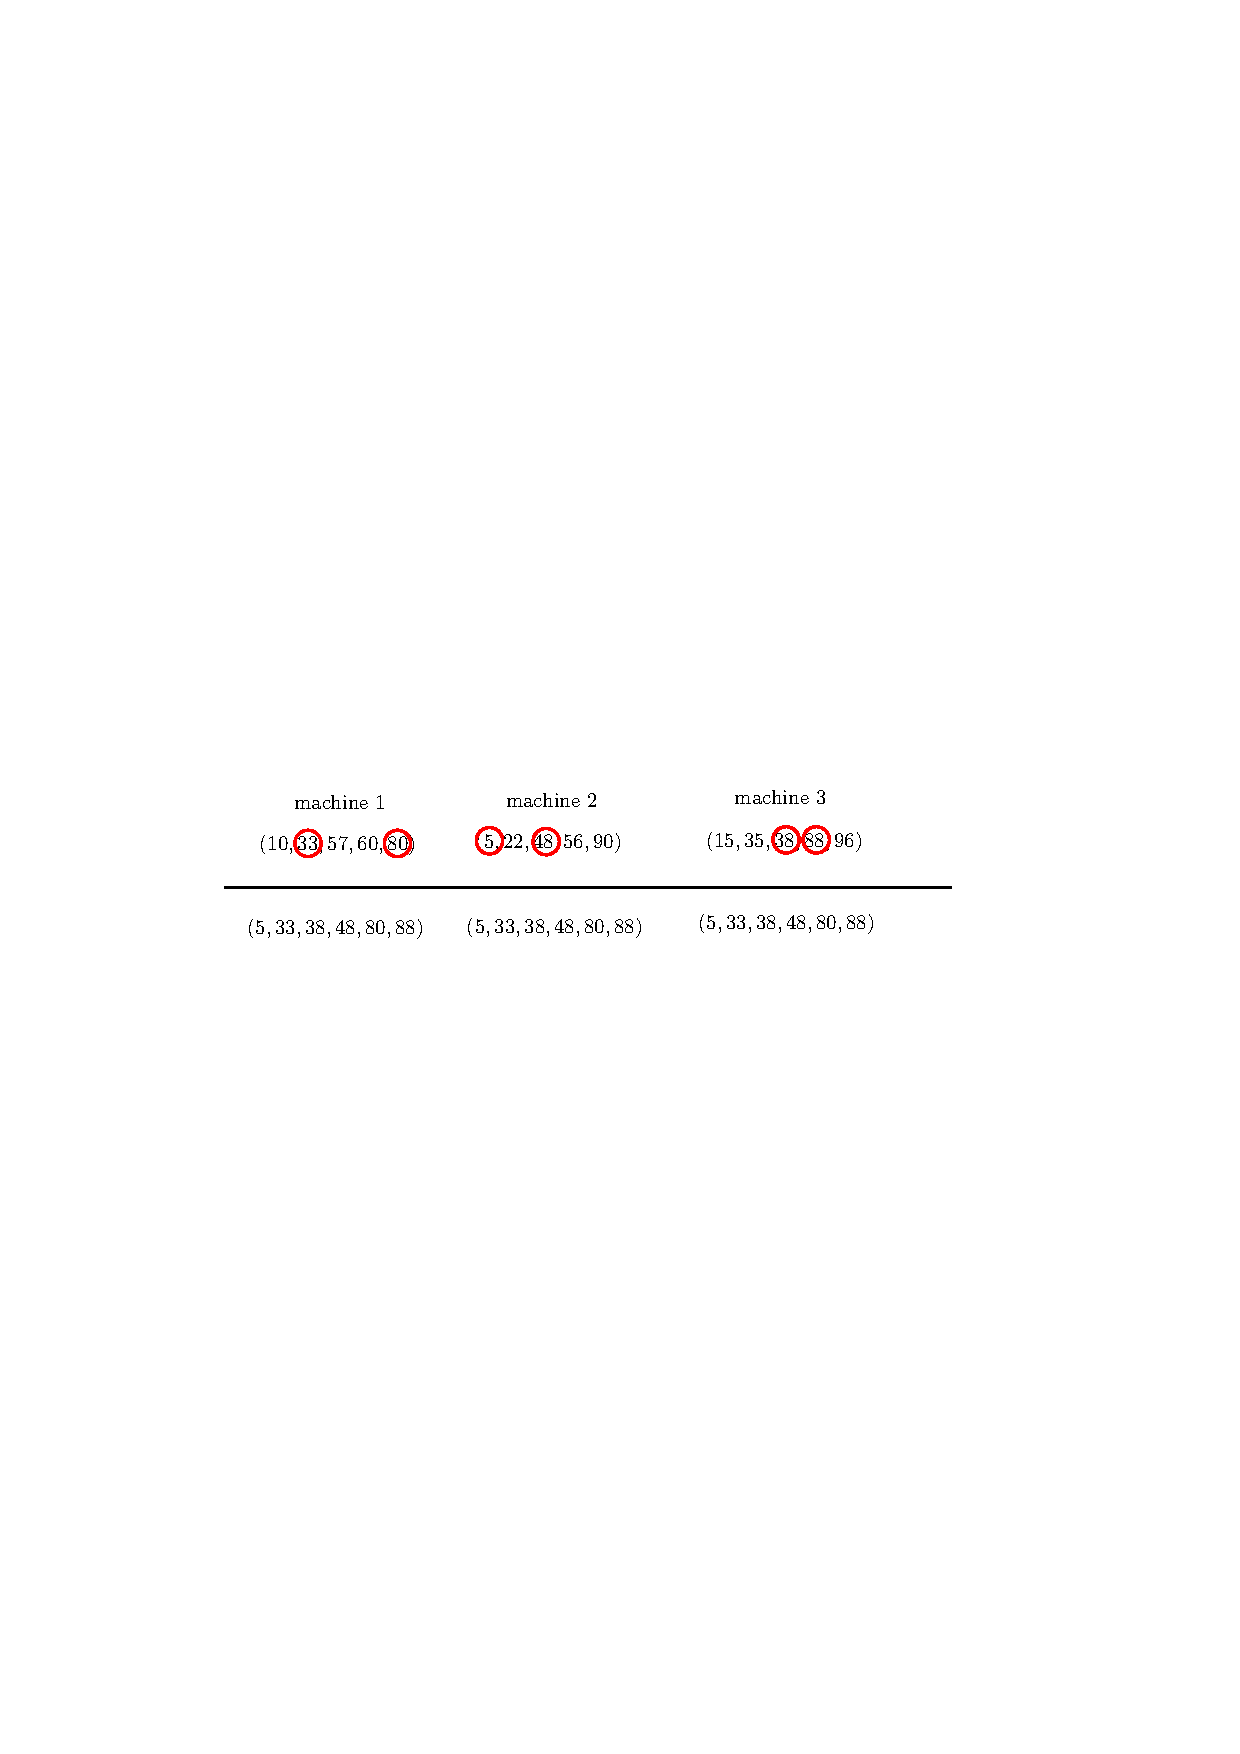
\includegraphics[height=20mm]{./artwork/tera}
    \end{center}


\end{small}
\end{frame}
%-------------------------------------------------------------

\begin{frame}
\begin{small}
    Let $\red{s}$ be the total number of samples (from all machines)

    \vgap

    \mybox[green]{Superstep 2}



    \begin{itemize}
        \item \blue{Step 1:} Each machine divides $\real$ into $p$ disjoint \blue{segments}, each covering at most $s / p$ samples. Let these segments be $\red{\sigma_1}, \red{\sigma_2}, ..., \red{\sigma_p}$ in ascending order.

    \begin{center}
        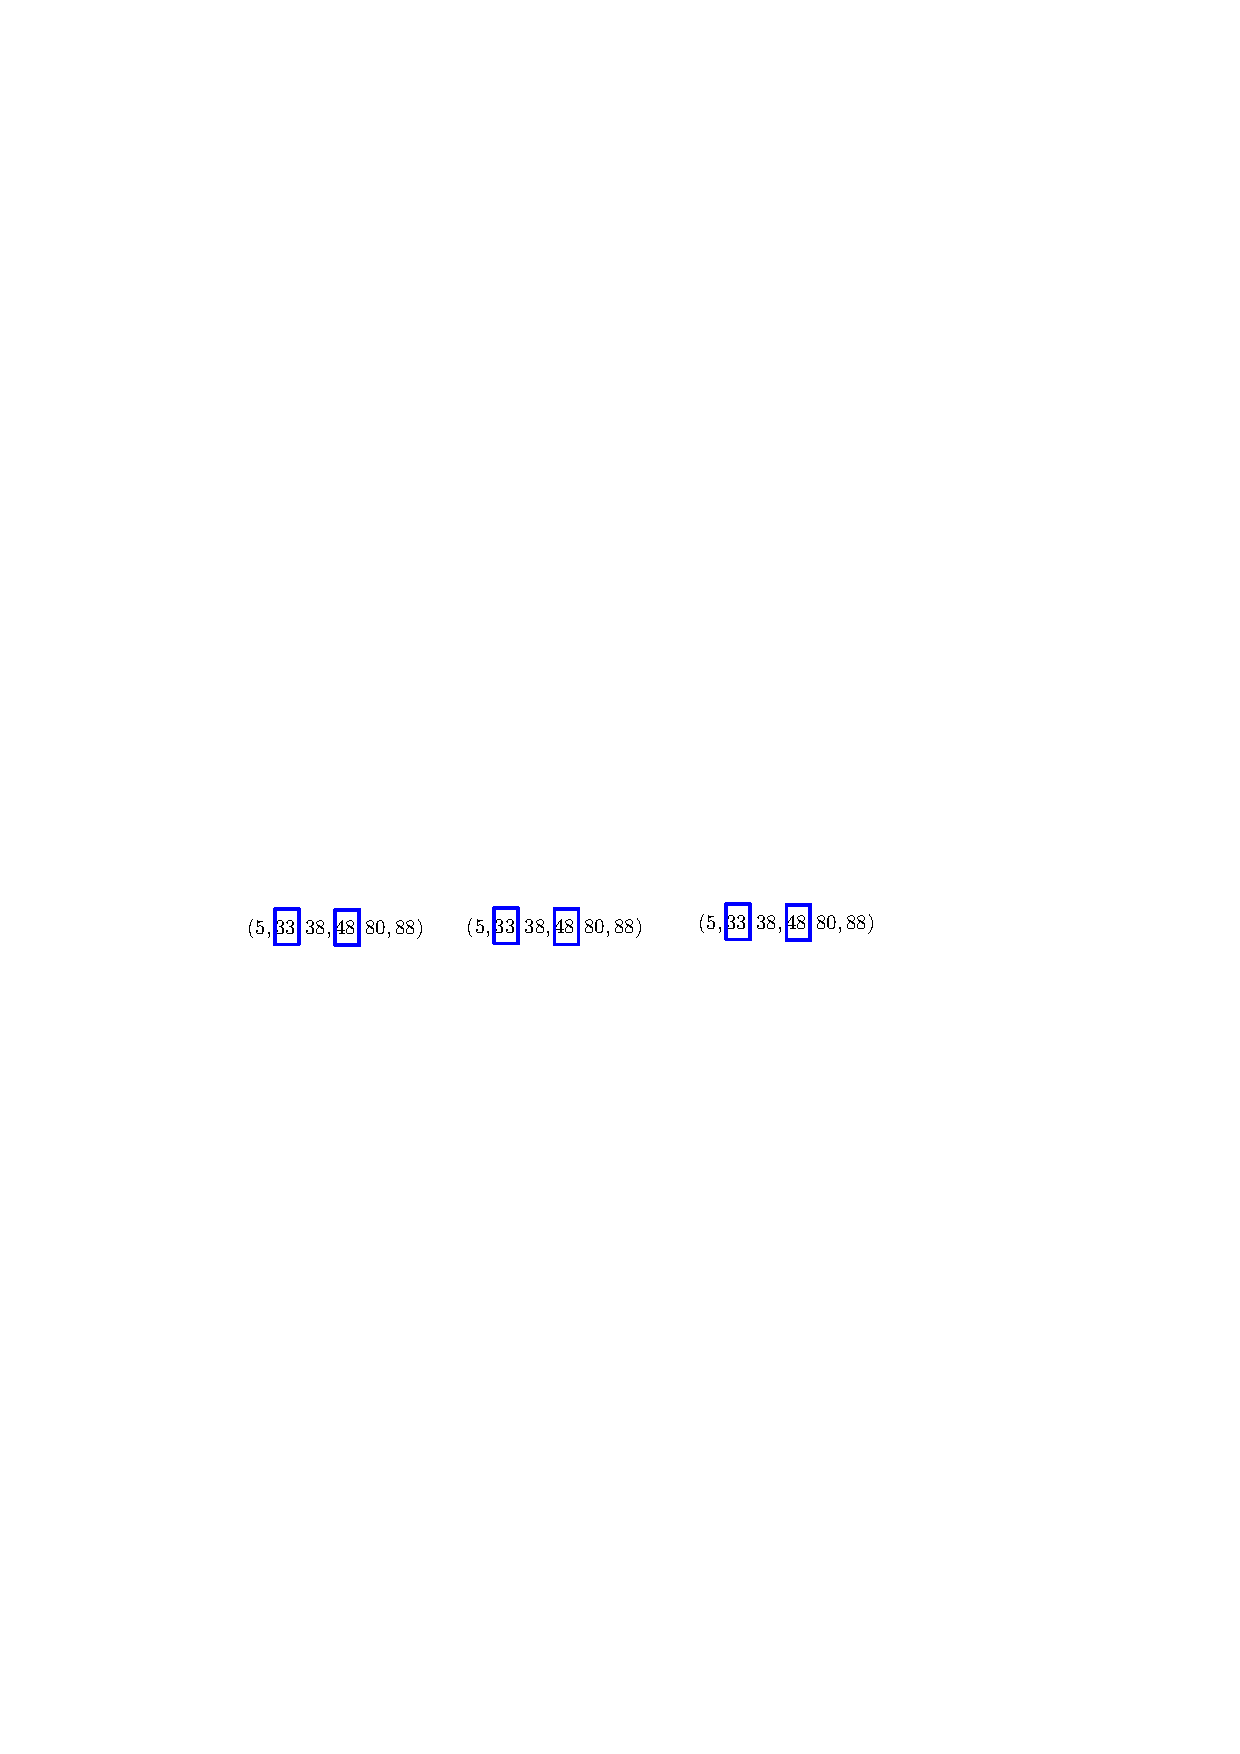
\includegraphics[height=5mm]{./artwork/tera0.5}
    \end{center}

        \item \blue{Step 2:} Machine $\red{i}$ sends $S_i \cap \sigma_j$ to machine $j$, for each $\red{j} \in [1, p]$.
    \end{itemize}

    \begin{center}
        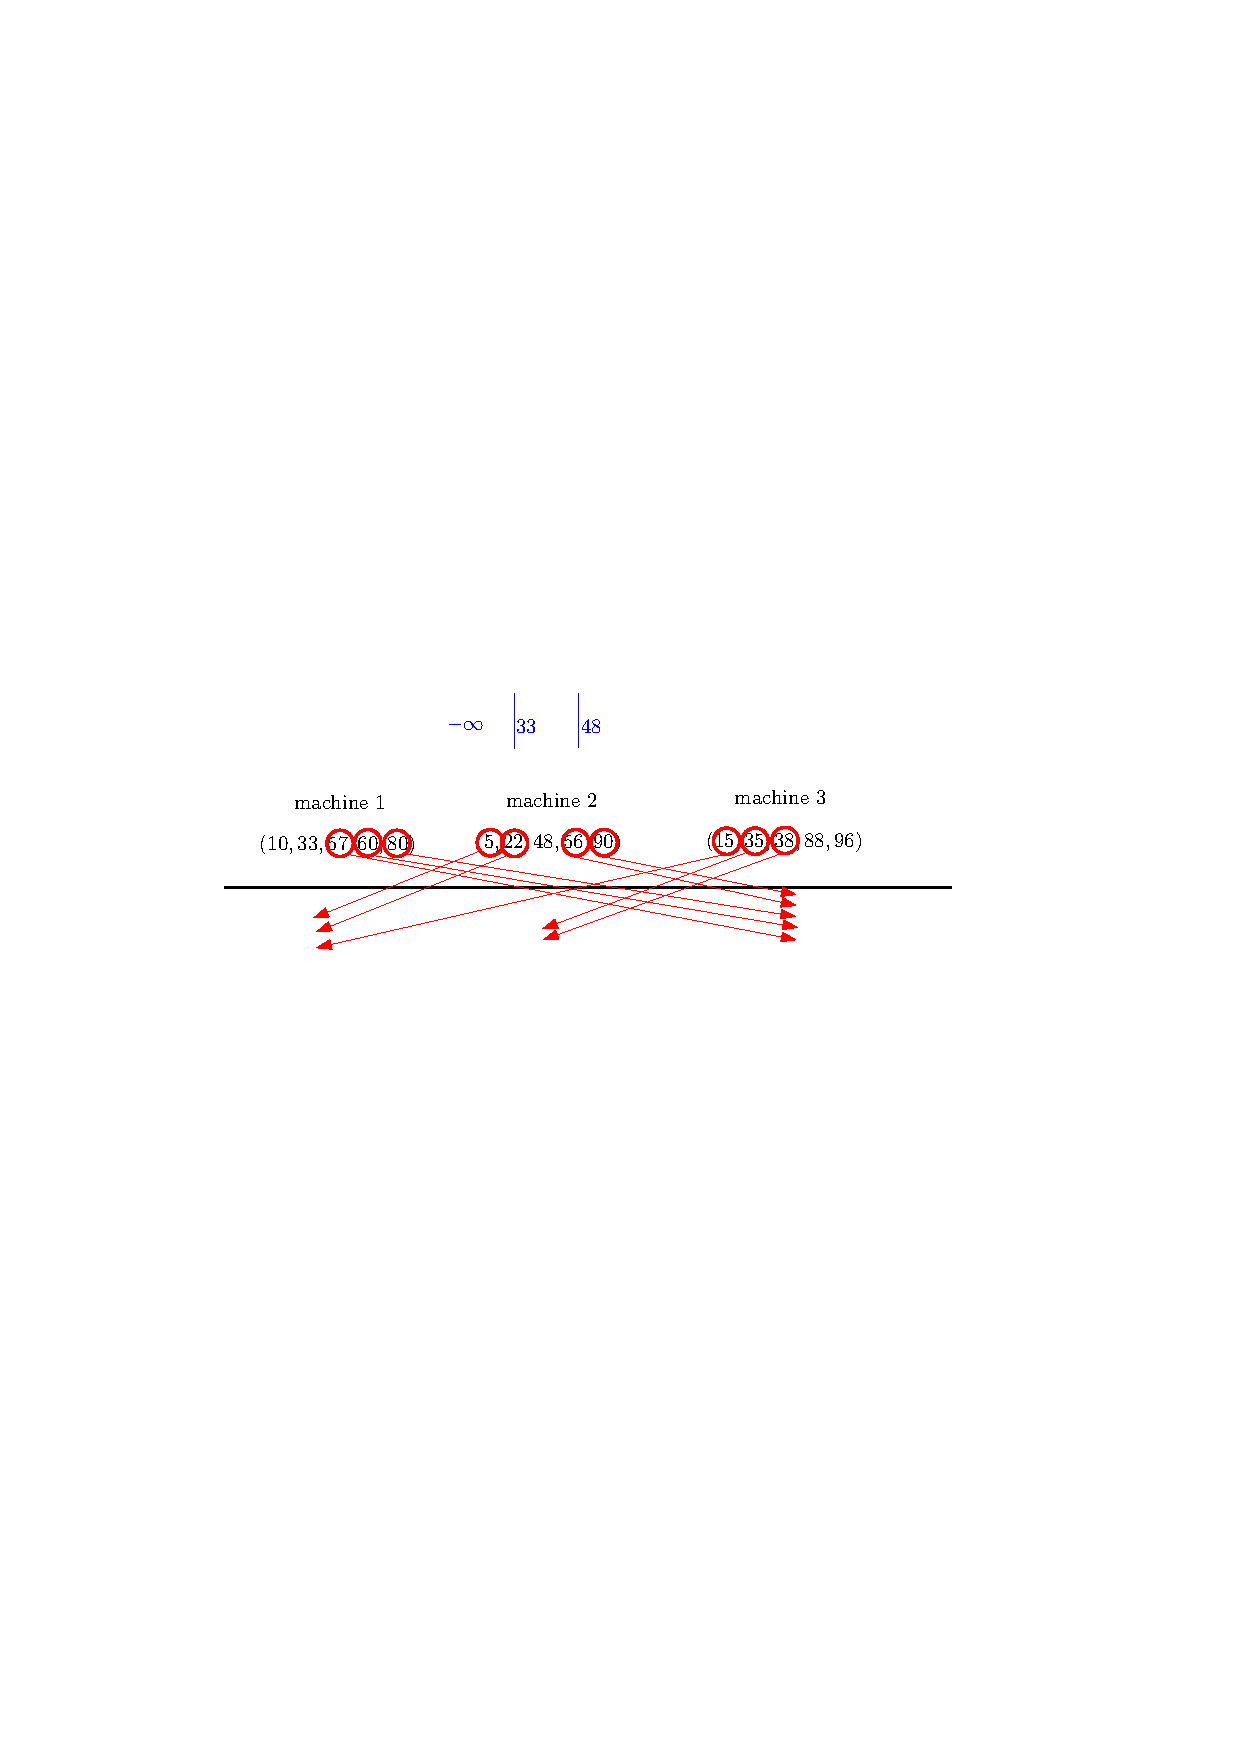
\includegraphics[height=35mm]{./artwork/tera1}
    \end{center}
\end{small}
\end{frame}
%-------------------------------------------------------------
\myfrm{
	We can prove that the cost of the algorithm is $O(n/p)$ with probability at least $1 - O(1/n)$.

	\vgap

	The proof is omitted from this talk.
}
%-------------------------------------------------------------
\end{document} 
